\documentclass[diploma]{softlab-thesis}
\setlength\parindent{0pt}
%\usepackage[greek,english]{babel}
%\usepackage{alphabeta}
%\usepackage{a4wide}

\usepackage{amssymb}
\usepackage{amsmath}
\usepackage{amsthm}
%\usepackage{amsfonts}
\usepackage{enumerate}
\usepackage{mathtools}

\usepackage{hyperref}

\usepackage{caption}
\usepackage{subcaption}
\usepackage{graphicx}

\usepackage[ruled]{algorithm2e}

\newcommand{\CC}{\vec{C}}
\newcommand{\Y}{\vec{Y}}
\newcommand{\x}{\vec{x}}
\newcommand{\y}{\vec{y}}
\newcommand{\g}{\gamma}
\newcommand{\xx}{\vec{x}\,'}
\newcommand{\A}{\mathcal{A}}


\counterwithin*{equation}{section}
\counterwithin*{equation}{subsection}

\newtheorem{theorem}{Theorem}[section]
\newtheorem{definition}{Definition}[section]
\newtheorem{lemma}{Lemma}[section]
\newtheorem{proposition}{Proposition}[section]
\newtheorem{obs}{Observation}[section]


\newtheorem{theoremgr}{Θεώρημα}[section]
\newtheorem{definitiongr}{Ορισμός}[section]
\newtheorem{lemmagr}{Λήμμα}[section]
\newtheorem{proofgr}{Απόδειξη}[section]

\setlength{\parindent}{1.5em}
\setlength{\parskip}{0.2em}

\begin{document}

\frontmatter


%%% TODO change
\title{Σχεδιασμός Μηχανισμών για Προβλήματα
Χωροθέτησης σε Ευσταθή Στιγμιότυπα}
\author{Αθηνά Τερζόγλου}
\date{Μάρτιος 2022}
%%% TODO change
\datedefense{22}{3}{2022}

\supervisor{Δημήτριος Φωτάκης}
\supervisorpos{Αν. Καθηγητής Ε.Μ.Π.}

%%% TODO change middle names?
\committeeone{Δημήτριος Φωτάκης}
\committeeonepos{Αν. Καθηγητής Ε.Μ.Π.}
\committeetwo{Αριστείδης Παγουρτζής}
\committeetwopos{Καθηγητής Ε.Μ.Π.}
\committeethree{Ευάγγελος Μαρκάκης}
\committeethreepos{Αν. Καθηγητής Ο.Π.Α}

%%% TODO change
%\TRnumber{CSD-SW-TR-42-18}  % number-year, ask nickie for the number
\department{Τομέας Τεχνολογίας Πληροφορικής και Υπολογιστών}

\maketitle


%%%  Abstract, in Greek

%%% TODO change
\begin{abstractgr}%
Σε αυτή τη διπλωματική, θα ασχοληθούμε με το σχεδιασμό μηχανισμών σε πρόβλημα χωροθέτησης υπηρεσιών, όπου $n$ στρατηγικοί παίκτες έχουν διαφορετικές προτιμήσεις σε ένα μετρικό χώρο. Ένας μηχανισμός είναι μία συνάρτηση που έχει ως είσοδο τις τοποθεσίες των παικτών και επιστρέφει ως έξοδο τις θέσεις των υπηρεσιών. Κάθε παίκτης έχει στόχο να ελαχιστοποιήσει το κόστος του, δηλαδή την απόσταση του από τη κοντινότερη υπηρεσία. Αυτό το δίνει το κίνητρό να δηλώσει διαφορετική τοποθεσία από τη πραγματική του. Για αυτό το λόγο ενδιαφερόμαστε για φιλαλήθης μηχανισμούς που εξασφαλίζουν ότι κανένας παίκτης δεν θα ωφεληθεί δηλώνοντας ψευδή τοποθεσία. Για να ξεπεράσουμε τη αδυναμία κατασκευής ντετερμινιστικού φιλαλήθη μηχανισμού με φραγμένο λόγο προσέγγισης, εστιάζουμε τη προσοχή μας σε ένα υποσύνολο στιγμιοτύπων που είναι ευσταθή σε διαταραχές. Η έννοια της ευστάθειας σε διαταραχές ορίστηκε πρώτη φορά σε προβλήματα \textit{Μέγιστης Τομής} και έπειτα σε προβλήματα Clustering. Με τα ευσταθή στιγμιότυπα μοντελοποιούμε τα στιγμιότυπα του ``πραγματικού κόσμου" στα οποία η βέλτιστη λύση δεν επηρεάζεται από μικρές διαταραχές στα  δεδομένα εισόδου. Αφού το πρόβλημα χωροθέτησης υπηρεσιών είναι πολύ στενά συνδεδεμένο με το clustering θέλουμε να δούμε πως μπορούμε να σχεδιάσουμε καλύτερους μηχανισμούς, αν υποθέσουμε ότι όλα τα πραγματικά στιγμιότυπα είναι ευσταθή. Δεδομένων των θετικών αποτελεσμάτων στη γραμμή, μας ενδιαφέρει να δούμε πως αυτά γενικεύονται και σε άλλους μετρικούς χώρους.
  
 
%%% TODO change
\begin{keywordsgr}
Προβλήματα Χωροθέτησης, Σχεδιασμός μηχανισμών χωρίς χρήματα, Κοινωνική Επιλογή, Ευστάθεια σε διαταραχές
\end{keywordsgr}
\end{abstractgr}


%%%  Abstract, in English

%%% TODO change
\begin{abstracten}%
In this thesis, we study $k$-Facility Location games, where $n$ strategic agents have different ideal locations on a metric space. A mechanism maps the locations reported by the agents to $k$ facilities. Each agent seeks to minimize her cost, namely the distance between her location and the nearest facility, which may incentivize her to misreport her location. Our goal is to design strategyproof (i.e, no agent can benefit by misreporting her location) mechanisms with a bounded approximation ratio to the optimal social cost. To overcome the impossibility results for deterministic strategyproof mechanisms, we restrict our attention in perturbation stable instances. The notion of perturbation stability was first introduced for the Max-Cut Problem and later was adapted for the Clustering Problems. This captures the ``real world" instances in which the optimal solution is well-defined and unaffected by small perturbation on the input. Since $k$-Facility Location games and $k$-Clustering are closely related problems, we are interested to see how perturbation stability can help us design strategyproof mechanisms with stronger guarantees. Given the recent results in $k$-Facility location in stable instances on the line, we are interested in extending those results in more general metric spaces. 
 
\begin{keywordsen}
Facility Location Games, Mechanism Design without Money, Social Choice, Perturbation Stability
\end{keywordsen}
\end{abstracten}


%%%  Acknowledgements

%%% TODO change
\begin{acknowledgementsgr}
Κατ' αρχάς θα ήθελα να ευχαριστήσω τον επιβλέποντα μου κ. Φωτάκη, που με ενέπνευσε να ασχοληθώ με το τομέα της Θεωρητικής Πληροφορικής και που πίστεψε στις δυνατότητες μου από την αρχή. Επίσης θα ήθελα να ευχαριστήσω τον Παναγιώτη Πατσιλινάκο για την εξαιρετική συνεργασία και τη βοήθεια κατά την εκπόνηση της διπλωματικής μου εργασίας. Τέλος, θα ήθελα να ευχαριστήσω την οικογένεια μου που με στήριξαν όλα αυτά τα χρόνια αλλά και τους φίλους μου που ήταν πάντα δίπλα μου σε αυτό το όμορφο ταξίδι.
\end{acknowledgementsgr}



\tableofcontents
\listoffigures
%\listoftables

%%%  Main part of the book

\mainmatter
\chapter{Εκτεταμένη Ελληνική Περίληψη}

\section{Εισαγωγή}

%Ένα από τα βασικότερα προβλήματα στις σύγχρονες κοινωνίες είναι οι συλλογικές αποφάσεις. Χαρακτηριστικό παράδειγμα αποτελούν οι εκλογές στις οποίες όλοι οι πολίτες καλούνται να δηλώσουν τον υποψήφιο που προτιμούν με σκοπό την επιλογή του συνολικά καλύτερου υποψηφίου. Αυτού του είδους τα προβλήματα έχουν μελετηθεί από τη σκοπιά της κοινωνιολογίας κυρίως, όμως πρόσφατα έχει μελετηθεί και από τη σκοπιά της επιστήμης των υπολογιστών. ++


Στη παρούσα διπλωματική εργασία θα ασχοληθούμε με το πρόβλημα της χωροθέτησης υπηρεσιών. Υποθέτουμε ότι ένα σύνολο παικτών βρίσκονται σε ένα χώρο και εμείς επιθυμούμε να τοποθετήσουμε υπηρεσίες σε διαφορετικές θέσεις στο χώρο αυτό. Το κόστος κάθε παίκτη είναι η απόσταση του από τη πλησιέστερη υπηρεσία. Στόχος μας είναι να βρούμε τις βέλτιστες θέσεις ώστε το συνολικό κόστος των παικτών να είναι όσο το δυνατόν μικρότερο. Το συγκεκριμένο πρόβλημα έχει μελετηθεί εκτενώς τόσο στο πεδίο της επιστήμης των υπολογιστών όσο και στο πεδίο της επιχειρησιακής έρευνας. Ο λόγος είναι ότι μοντελοποιεί πληθώρα προβλημάτων, όπως τη επιλογή των θέσεων χτισίματος καινούριων βιβλιοθηκών από την κυβέρνηση βάση των προτιμήσεων των πολιτών. 

Αν γνωρίζουμε τις πραγματικές τοποθεσίες των παικτών τότε μπορούμε να προσεγγίσουμε τη βέλτιστη λύση αρκετά καλά. Ωστόσο, υπάρχουν πολλές εφαρμογές που οι θέσεις των παικτών δεν είναι δημοσίως γνωστές και πρέπει να δηλώνονται στην κεντρική αρχή από στρατηγικούς παίκτες. Κάθε παίκτης έχει στόχο να ελαχιστοποιήσει το κόστος του, χωρίς να τον εδιαφέρει το συνολικό κόστος. Τώρα ο στόχος δεν είναι μόνο να βρούμε τις θέσεις των υπηρεσιών αλλά να τις βάλουμε με τέτοιο τρόπο που κανένας παίκτης δεν μπορεί να κερδίσει δηλώνοντας ψευδή τοποθεσία. Ενδιαφερόμαστε λοιπόν για το σχεδιασμό φιλαληθών μηχανισμών για για προβλήματα χωροθέτισης.

Σε πολλά προβλήματα σχεδιασμού μηχανισμών, όπως οι δημοπρασίες, εισάγουμε στο μοντέλο πληρωμές για να εγγυηθούμε ότι η ανάθεση των αγαθών γίνεται με φιλαλήθη τρόπο. Όμως, σε περιβάλλον κοινωνικής επιλογής όπως τα προβλήματα χωροθέτησης υπηρεσιών, μπορεί να είναι παράνομο ή ανήθικο να επιβάλουμε πληρωμές. Πάνω σε αυτή την ιδέα ξεκίνησε η εύρενα από τους rocaccia και Tennenholtz \cite{Procaccia2013} πάνω στο σχεδιασμό προσεγγιστικών μηχανισμών χωρίς χρήματα. 

\section{Προβλήματα Χωροθέτησης}

Πρώτα θα ορίσουμε το βασικό μοντέλο του προβλήματος. Έχουμε ένα μετρικό χώρο $(X,d)$, όπου $d:X \times X  \rightarrow \mathbb{R}_{+}$ είναι μια συνάρτηση απόστασης μεταξύ των σημείων του χώρου. Η συνάρτηση είναι μετρική που σημαίνει ότι $\forall x,y,z \in Z$: $d(x,x)=0$ (ταύτιση), $d(x,y)=d(y,x)$ (συμμετρία) και $d(x,z)\le d(x,y)+d(y,z)$ (τριγωνική ανισότητα). Οι παίκτες έχουν μια ιδανική τοποθεσία στον χώρο. Ένα στιγμιότυπο αποτελείται από τις θέσεις των παικτών στο χώρο $\x=(x_1,...,x_n)$. 


Κάθε παίκτης δηλώνει τη θέση του στο μηχανισμό $M$. Ένας ντετερμινιστικός μηχανισμός είναι μία συνάρτηση που απεικονίζει το σύνολο των δηλωθέντων θέσεων των παικτών $\x$ σε $k$ υπηρεσίες $(c_1,...,c_k)$. Αντίστοιχα ένας τυχαιοποιημένος μηχανισμός $M$ απεικονίζει το σύνολο των δηλωθέντων θέσεων των παικτών $\x$ σε μια πιθανοτική κατανομή από $k$ υπηρεσίες. $(c_1,...,c_k)$.  


 Tο κόστος κάθε παίκτη είναι η απόσταση του από τη πλησιέστερη υπηρεσία, $cost(x_i,M(\x)) = min_{1\le j \le k} \{d(x_i,c_j) \}$. Το κοινωνικό κόστος ενός μηχανισμού $M$ είναι το άθροισμα των κοστών των παικτών, $ cost(\x,M(\x)) = \sum_{i=1}^{n} cost(x_i,\CC)$.
 
 Κάθε παίκτης είναι στρατηγικός και έχει στόχο να ελαχιστοποιήσει το κόστος του. Ο μηχανισμός έχει στόχο να ελαχιστοποιήσει το κοινωνικό κόστος. Η διαφορά αυτή ωθεί τους παίκτες να δηλώσουν ψευδή τοποθεσία για να κερδίσουν. Για αυτό ενδιαφερόμαστε για φιλαλήθης μηχανισμούς που σημαίνει ότι κανένας παίκτης δεν μπορεί να κερδίσει λέγοντας ψέματα.
 
 Στη συνέχεια θα δούμε τα βασικά αποτελέσματα για προβλήματα χωροθέτησης υπηρεσιών. Πρώτα θα αναλύσουμε τη περίπτωση που οι παίκτες είναι τοποθετημένοι στη γραμμή και στη συνέχεια τη περίπτωση που οι παίκτες είναι τοποθετημένοι σε δέντρα.
 
 
 
 
\subsection*{Μια υπηρεσία στη γραμμή}

Όταν θέλουμε να τοποθετήσουμε μια υπηρεσία, η θέση του διάμεσου παίκτη είναι βέλτιστη και ταυτόχρονα είναι φιλαλήθης. Η βασική ιδέα είναι ότι ο μοναδικός τρόπος που ένας παίκτης μπορεί να αλλάξει τη θέση της υπηρεσίας είναι να δηλώσει μια θέση από τη ``άλλη" μεριά του διάμεσου. Αυτό, όμως, θα έχει ως αποτέλεσμα η υπηρεσία να πάει πιο μακριά σε σχέση με τη πραγματική του θέση. Άρα δεν υπάρχει τρόπος κάποιος παίκτης να κερδίσει λέγοντας ψέματα.

\begin{theoremgr}[\cite{Moulin1980}]
Ο μηχανισμός που τοποθετεί την υπηρεσία στο διάμεσο παίκτη είναι βέλτιστος και φιλαλήθης.
 \end{theoremgr}

\begin{figure}[ht]
    \centering
    
\includegraphics[width=0.6\textwidth]{Images/Median.png}
    \caption{Βέλτιστη λύση για μία υπηρεσία στη γραμμή}
    \label{fig:med}
\end{figure}

 
\subsection*{Δύο υπηρεσίες στη γραμμή}

Όταν θέλουμε να τοποθετήσουμε δύο υπηρεσίες το πρόβλημα γίνεται πιο δύσκολο. Αρχικά, μπορούμε εύκολα να δούμε ότι η βέλτιστη λύση δεν είναι φιλαλήθης. Μπορούμε να χωρίσουμε τους παίκτες σε δύο σύνολα, το δεξί και το αριστερό, ανάλογα με την υπηρεσία που προτιμούν. Όμως ένας παίκτης μπορεί να δηλώσει μια θέση που να τον βάζει στο άλλο σύνολο από αυτό που ανήκει πραγματικά, έτσι ώστε να φέρει την υπηρεσία του εκείνου του συνόλου πιο κοντά στην πραγματική του θέση. 


 
Ο μόνος τρόπος που μπορούμε να τοποθετήσουμε τις υπηρεσίες με φιλαλήθη τρόπο είναι να τις βάλουμε στο πιο δεξί και στον πιο αριστερό παίκτη. Παρατηρούμε ότι υποχρεωτικά ο πιο αριστερός παίκτης ανήκει στο αριστερό σύνολο και αντίστοιχα ο πιο δεξιά παίκτης ανήκει στο δεξί σύνολο. Με αυτό το τρόπο εξασφαλίζουμε φραγμένο λόγο προσέγγισης. Επιπλέον, τοποθετώντας τις υπηρεσίες στις ακριανές θέσεις παρατηρούμε ότι κανένας παίκτης δεν μπορεί να κερδίσει δηλώνοντας διαφορετική, αφού ο μόνος τρόπος να αλλάξει θέση μία υπηρεσία είναι να πάει πιο μακριά. 




\begin{figure}[ht]
    \begin{subfigure}[b]{\textwidth}
        \centering
        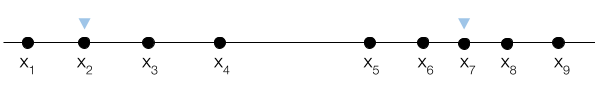
\includegraphics[width=0.8\textwidth]{Images/OPT2.png}
        \caption{Βέλτιστη ανάθεση}
        \label{fig:opt2}
     \end{subfigure}
    \hspace{20pt}
     \begin{subfigure}[b]{\textwidth}
        \centering
        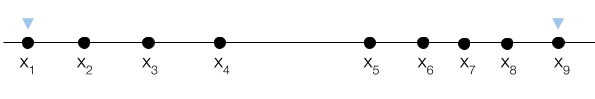
\includegraphics[width=0.8\textwidth]{Images/TwoExtremes.png}
        \caption{Ανάθεση στους δύο ακριανούς παίκτες}
        \label{fig:twoEx}
    \end{subfigure}
\end{figure}

\begin{theoremgr}[\textsc{Two Extremes  \cite{Procaccia2013}}]
Ο μηχανισμός που τοποθετεί τις υπηρεσίες στους δύο ακριανούς παίκτες είναι φιλαλήθης και έχει λόγο προσέγγισης $(n-2)$. 
\end{theoremgr}

Ο \textsc{Two Extremes} είναι ο μοναδικός ντετερμινιστικός μηχανισμός με φραγμένο λόγο προσέγγισης \cite{Fotakis2014}. Αν επιτρέψουμε στο μηχανισμό να χρησιμοποιήσει τυχαιότητα μπορούμε να πετύχουμε πολύ καλύτερο λόγο προσέγγισης. Ο proportional μηχανισμός είναι φιλαλήθης και έχει σταθερό λόγο προσέγγισης. Διαισθητικά τοποθετεί τη πρώτη υπηρεσία τυχαία σε μια από τις θέσεις των παικτών και τη δεύτερη τη τοποθετεί στη θέση κάποιου παίκτη με πιθανότητα ανάλογη της απόστασης του από τη πρώτη υπηρεσία.

\begin{definitiongr}[Propotional Μηχανισμός \cite{Lu2010}]
Για ένα στιγμιότυπο $\vec{x}=(x_1,...x_n)$, οι θέσεις των δύο υπηρεσιών επιλέγονται με τη παρακάτω τυχαία διαδικασία:
\begin{itemize}
    \item\textbf{Βήμα 1:} Επιλέγουμε ένα $i\in N$ τυχαία. Τοποθετούμε τη πρώτη υπηρεσία  $c_1$ στη θέση $x_i$

    \item\textbf{Βήμα 2:} Έστω $d_j = d(c_1,x_j)$ η απόσταση του παίκτη $j$ από τη πρώτη τοποθεσία. Επιλέγουμε το $j$ με πιθανότητα $\frac{d_j}{\sum_{k\in N}d_k}$. Τοποθετούμε τη δεύτερη υπηρεσία $c_2$ στη θέση $x_j$.
\end{itemize}
\end{definitiongr}

\begin{theoremgr} 
 O Proportional μηχανισμός είναι φιλαλήθης και έχει λόγο προσέγγισης το πολύ 4.
\end{theoremgr}

\subsection*{Περισσότερες από δύο υπηρεσίες στη γραμμή}

Όπως είδαμε το πρόβλημα γίνεται αρκετά πιο δύσκολο ακόμα και αν θέλουμε να τοποθετήσουμε μόνο δύο υπηρεσίες στη γραμμή. Δεν μπορούμε λοιπόν να περιμένουμε καλύτερα αποτελέσματα όταν θέλουμε να τοποθετήσουμε περισσότερες από δύο υπηρεσίες. Στη πραγματικότητα μπορούμε να δείξουμε ότι δεν υπάρχει ντετερμινιστικός φιλαλήθης μηχανισμός με φραγμένο λόγο προσέγγισης για $k\ge3$. Αυτό ισχύει ακόμα και για στιγμιότυπα με 4 παίκτες και 3 υπηρεσίες. Μπορούμε να δείξουμε ότι, όπως και πριν, οι δύο υπηρεσίες πρέπει να τοποθετηθούν στους δύο ακριανούς παίκτες για να είναι φιλαλήθης ο μηχανισμός. Η βασική ιδέα της απόδειξης είναι ότι δεν μπορούμε με φιλαλήθη τρόπο να επιλέξουμε σε ποιο παίκτη θα τοποθετηθεί η υπηρεσία. 

\begin{theoremgr}[\cite{Fotakis2014}]
Δεν υπάρχει ντερμινιστικός φιλαλήθης μηχανισμός με φραγμένο λόγο προσέγγισης για $k\ge3$.
\end{theoremgr}

Υπάρχει μια πολύ σημαντική οικογένεια ντετερμινιστικών μηχανισμών για προβλήματα χωροθέτησης. Διαισθητικά η οικογένεια των percentile μηχανισμών ``σπάει" το στιγμιότυπο σε τμήματα σύμφωνα με ένα διάνυσμα $\vec{p}$ και τοποθετεί μία υπηρεσία σε κάθε τμήμα. 

\begin{definitiongr}[$\vec{p}$-Percetntile Μηχανισμός \cite{Sui2013}]
    Ένας percentile μηχανισμός έχει ένα προκαθορισμένο διάνυσμα $\vec{p}=(p_1,...,p_k)$ τέτοιο ώστε $0\le p_1\le...\le p_k \le 1$. Ο μηχανισμός τοποθετεί τη $j$-οστή υπηρεσία στο $p_j$-οστό τμήμα του στιγμιότυπου. 
\[ c_j = x_{i_j}\; :\; i_j = \lfloor (n-1)\cdot p_j \rfloor +1 \]
\end{definitiongr}

Παράδειγμα του $(0.25,0.75)$-percentile μηχανισμού. Σε ένα στιγμιότυπο με 9 παίκτες ο μηχανισμός θα τοποθετεί τις υπηρεσίες στον 3ο παίκτη ($\lfloor 8\cdot 0.25 \rfloor +1  = 3$) και στον 7ο παίκτη ($\lfloor 8\cdot 0.75 \rfloor +1 = 7$), ανεξάρτητα από τις θέσεις των παικτών.
    \begin{center}
        
\includegraphics[width=0.8\textwidth]{Images/percentile.png}
    \end{center}

Αυτοί οι μηχανισμοί είναι φιλαλήθης για κάθε $k\ge2$. Είναι πολύ σημαντικό να σημειώσουμε ότι το διάνυσμα είναι προκαθορισμένο και δεν εξαρτάται από το στιγμιότυπο. Αυτός είναι και ο λόγος που είναι φιλαλήθης οι μηχανισμοί. Οι υπηρεσίες τοποθετούνται σε συγκεκριμένες θέσεις στο στιγμιότυπο ανεξάρτητα από τις θέσεις των παικτών. Ο μόνος τρόπος κάποιος παίκτης να αλλάξει τη θέση μια υπηρεσίας είναι να δηλώσει τοποθεσία σε άλλο τμήμα. Όπως στη μία υπηρεσία και το διάμεσο παίκτη, αυτή η αλλαγή θα πάει την υπηρεσία πιο μακριά. Το μειονέκτημα αυτών των μηχανισμών είναι ότι δεν έχουν πεπερασμένο λόγο προσέγγισης για $k\ge3$, όπως μας υποδηλώνει και το προηγούμενο θεώρημα. Ο μόνος percentile μηχανισμός με φραγμένο λόγο προσέγγισης είναι ο $(0,1)$-percentile μηχανισμός που είναι ισοδύναμος με τον \textsc{Two Extremes} μηχανισμό. Σε κάθε άλλη περίπτωση μπορούμε να δημιουργήσουμε ένα στιγμιότυπο στο οποίο οι παίκτες που έχουν υπηρεσίες στις θέσεις τους να είναι κοντά μεταξύ τους ενώ οι παίκτες που δεν έχουν υπηρεσίες να είναι μακριά. Αφού οι μηχανισμοί δεν ``κοιτούν" το στιγμιότυπο θα έχουν πολύ κακό λόγο προσέγγισης.

Είναι πολύ σημαντικό να παρατηρήσουμε ότι ο μόνος τρόπος για να έχουμε φραγμένο λόγο προσέγγισης είναι να τοποθετήσουμε μια υπηρεσία σε κάθε βέλτιστο cluster, δηλαδή σε κάθε ομάδα που εξυπηρετείται από την ίδια υπηρεσία στη βέλτιστη λύση. Όμως αυτό δεν μπορούμε να το πετύχουμε με φιλαλήθη τρόπο διότι η δομή των ομάδων αλλάζει όταν ένας παίκτης δηλώνει ψευδή τοποθεσία. Αυτό το εκμεταλλεύονται οι παίκτες για να κερδίσουν. Αν, από την άλλη, θέλουμε να έχουμε φιλαλήθης μηχανισμούς δεν πρέπει να ``κοιτάμε" τη δομή των ομάδων χάνοντας όμως το πεπερασμένο λόγο προσέγγισης. 

Από την άλλη πλευρά, μπορούμε να πετύχουμε καλύτερα αποτελέσματα αν επιτρέψουμε στους μηχανισμούς να χρησιμοποιήσουν τυχαιότητα. Πρώτα προτάθηκε ο  \textsc{Inversely Proportional Μηχανισμός} \cite{escoffier2011}, ο οποίος είναι $n/2$-προσεγγιστικός για $k$-υπηρεσίες με $n=k+1$ παίκτες. Έπειτα, προτάθηκε ο \textsc{Equal Cost} \cite{Fotakis2013sp} για $k$ υπηρεσίες και αυθαίρετο αριθμό παικτών, ο οποίος πετυχαίνει λόγο προσέγγισης το πολύ $n$. 


\begin{table}[ht]
    \centering
    \begin{tabular}{|c|c|c|c|}
         \hline
         & $k=1$ & $k=2$ & $k\ge3$ \\ \hline 
        Ντερμινιστικός & 1\cite{Moulin1980} & $n-2$ \cite{Procaccia2013} & $\infty$ \cite{Fotakis2013}\\ \hline
        Τυχαιοποιημένος & 1\cite{Moulin1980} & 4 \cite{Lu2010} & $n$ \cite{Fotakis2013sp} \\ \hline
    \end{tabular}
    \caption{Συγκεντρωτικός πίνακας των καλύτερων λόγων προσέγγισης για προβλήματα χωροθέτησης $k$ υπηρεσιών στη γραμμή.}
    \label{tab:summaryLineGr}
\end{table}


\subsection*{Τοποθέτηση υπηρεσιών σε δέντρα}

Τα δέντρα είναι ένας πιο γενικός μετρικός χώρος από τη γραμμή, με παρόμοιες ιδιότητες. Όταν θέλουμε να τοποθετήσουμε μια υπηρεσία, όπως και στη γραμμή, η βέλτιστη λύση είναι φιλαλήθης.

\begin{theoremgr}[\cite{Schummer2002}]
Ο μηχανισμός που τοποθετεί την υπηρεσία στο διάμεσο παίκτη είναι φιλαλήθης και βέλτιστος για το κοινωνικό κόστος.
\end{theoremgr}


Η βασική ιδέα είναι ίδια με τη γραμμή. Ο μόνος τρόπος ένας παίκτης να αλλάξει τη θέση της υπηρεσίας είναι να δηλώσει ότι η θέση του είναι από την άλλη μεριά του διαμέσου. Έτσι όμως η υπηρεσία πηγαίνει πιο μακριά.

Αν όμως θέλουμε να τοποθετήσουμε δύο υπηρεσίες το πρόβλημα γίνεται πολύ πιο δύσκολο. Αρχικά να σημειώσουμε ότι η έννοια του πιο δεξιού και του πιο αριστερού παίκτη δεν μεταφέρεται στα δέντρα. Μπορούμε να δείξουμε ότι ακόμα και όταν δέντρο αποτελείται από κλαδιά (3 ημιευθείες $[0,\infty)$ με κοινή αρχή), δεν υπάρχει ντετερμινιστικός μηχανισμός για τη τοποθέτηση δύο υπηρεσιών \cite{Fotakis2014}.




\section{Ευστάθεια σε Διαταραχές σε προβλήματα Συσταδοποίησης}

Τους περισσότερους αλγορίθμους τους χαρακτηρίζουμε βάση της επίδοσης τους στο χειρότερο πιθανό στιγμιότυπο. Αν και είναι πολύ σημαντικό εργαλείο στην κατανόηση της απόδοσης ενός αλγορίθμου έχει και κάποια αρνητικά χαρακτηριστικά. Ένα από τα κυριότερα είναι ότι τα χειρότερα στιγμιότυπα, που μπορεί να επηρεάζουν σημαντικά την απόδοση του αλγορίθμου, δεν είναι πιθανό να εμφανιστούν στον πραγματικό κόσμο. Για αυτό, τα τελευταία χρόνια η έρευνα έχει στραφεί στην ανάλυση πέρα της χειρότερης περίπτωσης. Υπάρχουν διαφορετικές τεχνικές μέσα από τις οποίες μπορούμε μελετήσουμε τη μέση περίπτωση. Εμείς θα ασχοληθούμε κυρίως με την ``ευστάθεια σε διαταραχές". Σε αυτό το μοντέλο θεωρούμε ότι η βέλτιστη λύση είναι καλά ορισμένη, που σημαίνει ότι δεν επηρεάζεται από μικρές αλλαγές στην είσοδο του προβλήματος. Με αυτό το τρόπο διαχωρίζουμε τα στιγμιότυπα που αξίζει να μελετήσουμε, αυτά δηλαδή που εμφανίζονται στη πράξη, από αυτά που δεν αξίζει.

Πιο συγκεκριμένα θα μελετήσουμε το πρόβλημα συσταδοποίησης σε ευσταθή στιγμιότυπα. Στο πρόβλημα συσταδοποίησης σκοπός είναι να χωρίσουμε ένα σύνολο σημείων του χώρου σε ομάδες, ώστε τα σημεία που ανήκουν στην ίδια ομάδα να είναι ``όμοια" ενώ τα σημεία σε διαφορετικές ομάδες να είναι ``διαφορετικά". Αυτό είναι ένα από τα πολύ γνωστά $NP$-hard προβλήματα. Παρόλα αυτά, σε ευσταθή στιγμιότυπα μπορούμε να βρούμε αποδοτικά τη βέλτιστη λύση. 


 
\begin{definitiongr}[$k$-Συσταδοποίηση  (Clustering)]
Για ένα σύνολο σημείων $X$ και μία μη-αρνητική συνάρτηση $d: X\times X \rightarrow [ 0, \infty )$ το clustering $\vec{C} = (C_1,C_2,...,C_k)$ είναι ο διαχωρισμός των σημείων σε $k$ μη-κενά σύνολα με κέντρα $c_1,...,c_k$ τα οποία ελαχιστοποιούν  το άθροισμα των αποστάσεων των σημείων από τα κέντρα τους (The $k$-median objective):
    \[ \sum_{i=1}^{k} \left( \sum_{x\in C_i}  d(c_i,x)\right) \]
    
\end{definitiongr}

Όπως περιγράψαμε και παραπάνω τα ευσταθή στιγμιότυπα του clustering είναι αυτά στα οποία η βέλτιστη λύση δεν επηρεάζεται από αλλαγές στην είσοδο. Ο μαθηματικός τρόπος να ορίσουμε αυτές τις ``αλλαγές" είναι να δημιουργήσουμε κοντινά στιγμιότυπα στα οποία ένα υποσύνολο των αποστάσεων μεταξύ δύο σημείων έχει μειωθεί κατά ένα παράγοντα $\g$, με $\g\ge1$. Άρα θα λέμε ένα στιγμιότυπο ευσταθές αν η βέλτιστη λύση παραμένει η ίδια σε κάθε πιθανό κοντινό στιγμιότυπο.


\begin{definitiongr}[$\g$-διαταραχή]
Για $\g \ge$  1, μια $\g$-διαταραχή ενός μετρικού χώρου $(X, d)$ είναι ένας άλλος χώρος $(X, d')$ πάνω στα ίδια σημεία τέτοιος ώστε:
\[ d'(x,y) \in \left[\frac{1}{\g}d(x,y),d(x,y)\right] \]
\end{definitiongr}



\begin{definitiongr}[$\g$-ευστάθεια] 
Ένα στιγμιότυπο $(X, d)$ είναι $\g$-ευσταθές για μία αντικειμενική συνάρτηση $\Phi$ αν υπάρχει ένα  k-clustering $\vec{C}= C_1, . . . , C_k$ τέτοιο ώστε, για κάθε $\g$-διαταραχή $(X, d')$, το  $\vec{C}$ να παραμένει το μοναδικό βέλτιστο  k-clustering.
\end{definitiongr}

Βάση αυτού του ορισμού προκύπτουν 3 σημαντικές ιδιότητες για τις αποστάσεις μεταξύ σημείων από διαφορετικό cluster.

\begin{definitiongr}[$\g$-Center Proximity]
Για κάποιο $\g \ge 1$, ένα $\g$-ευσταθές στιγμότυπο με μοναδικό βέλτιστο clustering $C_1, . . . , C_k$ και βέλτιστα κέντρα $c_1, . . . , c_k$ ικανοποιεί το $\g$-center proximity. Για δύο διαφορετικά cluster $C_i$ και $C_j$ και κάποιο σημείο $x_i\in C_i$: 
\[d(x_i,c_j)>\g d(x_i,c_i) \]
\end{definitiongr}

\begin{lemmagr}[$\g$-Weak Center Proximity]
Για $\g \ge 2$, ένα $\g$-ευσταθές στιγμότυπο με μοναδικό βέλτιστο clustering $C_1, . . . , C_k$ και βέλτιστα κέντρα $c_1, . . . , c_k$ ικανοποιεί το $\g-$weak center proximity. Για κάποιο $x\in C_i$ και $y \notin C_i$:
\[d(x,y)>(\g -1) d(x,c_i) \]
\end{lemmagr}

\begin{lemmagr}[Cluster Separation Property]

Έστω $C_1, . . . , C_k$ το μοναδικό βέλτιστο clustering ενός $\g$-ευσταθούς στιγμιοτύπου με  $\g\ge2$. Για  τα $x_i,x_i'\in C_i$ και το $x_j \in C_j$ $(i\ne j)$ ισχύει:
\[ d(x_i,x_j) > \frac{(\g-1)^2}{2\g} d(x_i,x_i') \]
\end{lemmagr} 

Για το clustering ένας από τους πιο συχνά χρησιμοποιόυμενους αλγορίθμους είναι ο single-linkage. Ξεκινάει με $n$ cluster (τα σημεία) και σε κάθε βήμα ενώνει τα δύο πιο ``κοντινά" cluster, μέχρις ότου μείνουν $k$ cluster. Για αυτό το παράδειγμα θεωρούμε ότι η απόσταση δύο clusters δίνεται από την ελάχιστη απόσταση ενός σημείου από το ένα cluster και ενός σημείου από το άλλο. Βλέπουμε ότι αυτός ο αλγόριθμος βασίζεται στις αποστάσεις μεταξύ των σημείων. Αν το στιγμιότυπο είναι ευσταθές μπορεί αυτός ο αλγόριθμος να βρει τη βέλτιστη λύση; Υπάρχει ένα απλό αντιπαράδειγμα που αυτός ο αλγόριθμος αποτυγχάνει. Ας υποθέσουμε ότι έχουμε ένα στιγμιότυπο με 4 διαφορετικές τοποθεσίες, έστω $\x=(x_1,x_2,x_3,x_4)$, ένας παίκτης είναι στη τοποθεσία $x_1$ και $M$ παίκτες σε κάθε μία από τις υπόλοιπες. Στόχος μας είναι να τοποθετήσουμε 3 υπηρεσίες.   
\begin{figure}[ht]
    \centering
    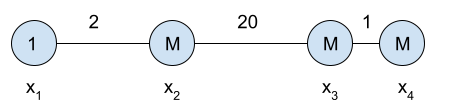
\includegraphics[width=0.6\textwidth]{Images/SingleLinkageC.png}
    \caption{Αντιπαράδειγμα του single-linkage}
    \label{fig:singleGR}
\end{figure}

Είναι εύκολο να δούμε ότι η βέλτιστη λύση είναι να τοποθετήσουμε τα κέντρα στις θέσεις $x_2$,$x_3$ και $x_4$ και να εξυπηρετήσουμε τον $x_1$ από το κέντρο στο $x_2$. Το συνολικό κόστος της βέλτιστης λύσης είναι 2. Όμως ο single-linkage θα ενώσει σε ένα cluster τις θέσεις $x_3$ και $x_4$. Αυτή η λύση όμως έχει κόστος $M$.

Με μία μικρή τροποποίηση στον παραπάνω αλγόριθμο μπορούμε να παίρνουμε πάντα τη βέλτιστη λύση σε ευσταθή στιγμιότυπα. Αντί να σταματάμε στα $k$ clusters συνεχίζουμε μέχρι να μείνει ένα cluster και στη συνέχεια με δυναμικό προγραμματισμό μπορούμε να βρούμε το βέλτιστο $k$-clustering.

\begin{lemmagr} 
O single-linkage αλγόριθμος βρίσκει πάντα τη βέλτιστη λύση αν, και μόνο αν, κάθε βέλτιστο cluster είναι υποδέντρο του ελάχιστου συνεκτικού δέντρου.
\end{lemmagr}

\begin{figure}[ht]
    \centering
    
\includegraphics[width=0.5\textwidth]{Images/MSTconnected.png}
    \caption{Τα βέλτιστα cluster είναι υποδέντρα του ΕΣΔ.}
    \label{fig:MSTCon}
\end{figure}

Το παραπάνω λήμμα ισχύει διότι o single-linkage μπορεί να φτιάξει $k$-clusterings αφαιρώντας $k-1$ ακμές από το δέντρο. Αν τα clusters δεν είναι υποδέντρα δεν υπάρχει τρόπος να τα φτιάξει.

\begin{lemmagr}[\cite{Angelidakis2017}]
Ο single-linkage βρίσκει τη βέλτιστη λύση για κάθε 2-ευσταθές στιγμιότυπο.  
\end{lemmagr}


\section{Προβλήματα Χωροθέτησης σε Ευσταθή Στιγμιότυπα}

Όπως είδαμε και παραπάνω η βασική δυσκολία των προβλημάτων χωροθέτησης είναι:
\begin{enumerate}[(i)]
    \item Αν θέλουμε φραγμένο λόγο προσέγγισης πρέπει να τοποθετήσουμε τις υπηρεσίες βάση των αποστάσεων μεταξύ των παικτών. Έτσι όμως οι μηχανισμοί δεν είναι φιλαλήθης. 
    \item  Αν θέλουμε φιλαλήθης μηχανισμούς δεν πρέπει να ``κοιτάμε" το στιγμιότυπο. Έτσι όμως οι μηχανισμοί δεν έχουν φραγμένο λόγο προσέγγισης.
\end{enumerate}

Αν όμως υποθέσουμε ότι τα πραγματικά στιγμιότυπα είναι ευσταθή, μπορούμε να σχεδιάσουμε μηχανισμούς με καλύτερες εγγυήσεις; Τα βέλτιστα cluster στα ευσταθή στιγμιότυπα είναι εύκολα διαχωρίσιμα που σημαίνει ότι μπορούμε να τοποθετήσουμε μία υπηρεσία σε κάθε βέλτιστο cluster για να έχουμε φραγμένο λόγο προσέγγισης αλλά ταυτόχρονα οι παίκτες έχουν λιγότερη δύναμη στο να αλλάξουν τα βέλτιστα cluster. Αξίζει να σημειώσουμε ότι αυτό δεν είναι εφικτό χωρίς να υποθέσουμε ότι το στιγμιότυπο είναι ευσταθές, ακόμα και δύο υπηρεσίες στη γραμμή.

%Αν υποθέσουμε ότι το στιγμιότυπο είναι ευσταθές, μπορούμε να χρησιμοποιήσουμε τη δομή που έχει για να σχεδιάσουμε καλύτερους μηχανισμούς. 
Η βασική διαφορά μεταξύ της προηγούμενης ενότητας και αυτής είναι ότι οι παίκτες είναι στρατηγικοί. Κάθε παίκτης έχει το δικαίωμα να δηλώσει οποιαδήποτε θέση επιθυμεί ανεξάρτητα από τη πραγματική του. Αντίθετα, οι διαταραχές που χρησιμοποιούμε για να δείξουμε ότι ένα στιγμιότυπο είναι ευσταθές παράγονται με συγκεκριμένο τρόπο. Από εδώ και πέρα, θα υποθέσουμε ότι τα πραγματικά στιγμιότυπα που θα έχει να χειριστεί ένας μηχανισμός είναι ευσταθή και θα μελετήσουμε τη δύναμη που έχει ένας παίκτη να αλλάξει την έξοδο του μηχανισμού. 

%\begin{definitiongr}[$\g$-διαταραχή και $\g$-ευστάθεια]

%\end{definitiongr}
Για τα ευσταθή στιγμιότυπα έχουμε δύο πολύ σημαντικές ιδιότητες που θα μας φανούν πολύ χρήσιμες στη συνέχεια.

\begin{lemmagr}\label{con}
Έστω ένα $\g$-ευσταθές στιγμιότυπο $\x$, με $\g\ge2$. Τότε κάθε βέλτιστο cluster είναι υποδέντρο του δέντρου.
\end{lemmagr}

\begin{lemmagr}
Έστω ένα $\g$-ευσταθές στιγμιότυπο, με $\g\ge2+\sqrt{3}$. Από το cluster separation property έχουμε ότι για κάθε τοποθεσία $x_i$ κάθε εσωτερική απόσταση είναι μικρότερη από κάθε εξωτερική:
\[ d(x_i,x_j) \ge d(x_i,x_i') \; \forall x_i,x_i;\in C_i \;\&\; x_j \in C_j\]
\end{lemmagr}

Μια αρνητική παρατήρηση για τη βέλτιστη λύση είναι ότι δεν είναι φιλαλήθης αν περιέχει έστω και ένα cluster με ένα μόνο παίκτη (singleton cluster). Ας υποθέσουμε ότι το πραγματικό στιγμιότυπο είναι αυτή της εικόνας \ref{fig:original}. Αν ένας παίκτης δηλώσει μια θέση ``πολύ μακριά" από τους υπόλοιπους παίκτες τότε θα έχει μια υπηρεσία στη θέση που δήλωσε ενώ το υπόλοιπο στιγμιότυπο θα εξυπηρετηθεί από $k-1$ υπηρεσίες. Όπως φαίνεται και στη εικόνα \ref{fig:deviation} τα δύο cluster θα ενωθούν και έτσι ο παίκτης που δήλωσε ψευδή θέση κατάφερε να φέρει μια υπηρεσία πιο κοντά στη πραγματική του θέση. Το πρόβλημα είναι ότι και τα δύο στιγμιότυπα είναι $\g$-ευσταθή και δεν μπορούμε με κάποιο τρόπο να διαχωρίσουμε αν το στιγμιότυπο είναι πραγματικό ή αν έχει προκύψει από κάποια αλλαγή. Παρόλα αυτά, στα πραγματικά στιγμιότυπα που μοντελοποιούν προβλήματα χωροθέτησης υπηρεσιών είναι φυσικό να υποθέσουμε ότι δεν υπάρχουν singleton clusters. 



\begin{figure}[ht]
\centering
    \begin{subfigure}[b]{0.35\textwidth}
         \centering
         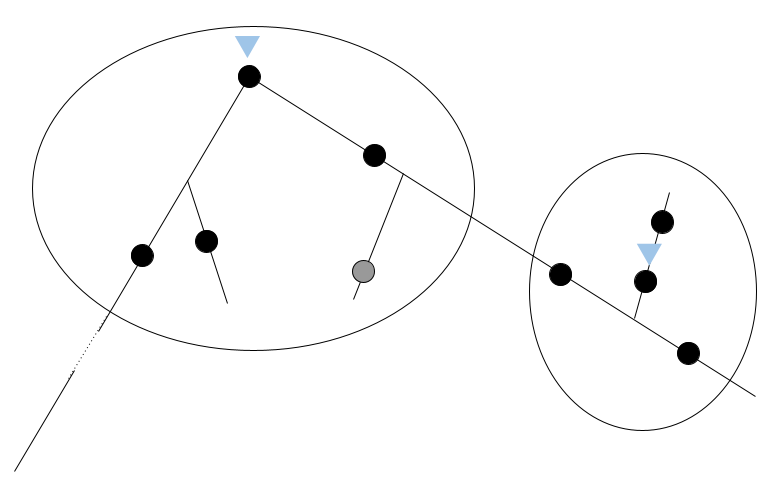
\includegraphics[width=\textwidth]{Images/stable1.png}
         \caption{Αρχικό στιγμιότυπο}
         \label{fig:original}
     \end{subfigure}
    \hspace{50pt}
    \begin{subfigure}[b]{0.35\textwidth}
         \centering
         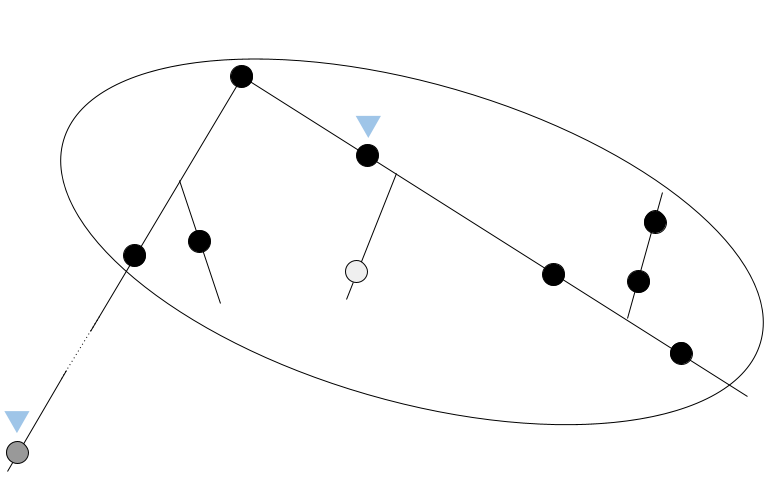
\includegraphics[width=\textwidth]{Images/stable2.png}
         \caption{Το στιγμιότυπο μετά την αλλαγή.}
         \label{fig:deviation}
     \end{subfigure}
    \end{figure}

\begin{algorithm}[ht]
\label{algorithm:optimalgr}
\DontPrintSemicolon
\SetAlgoLined
\LinesNumbered
\KwResult{Μια ανάθεση $k$-υπηρεσιών}
\KwIn{Ένα στιγμιότυπο $\x$ $k$-Facility Location.}
Υπολογισμός του βέλτιστου clustering
 $(C_1, \ldots, C_k)$. Έστω $c_i$ η διάμεση θέση του cluster $C_i$.\;

 \uIf{\big($\exists i \in [k]$ with $|C_i|=1$\big) or \big($\exists \;x_i,x_i'\in Ci$ and  $x_j,x_j'\in C_j$ with $\max\{ d(x_i,x_i'), d(x_j,x_j')\} \geq d(x_i,x_j) $\big)}{
 \KwOut {``Δεν τοποθετούνται υπηρεσίες''.}}\uElse{
 
\KwOut {Οι $k$-υπηρεσίες τοποθετούνται στις θέσεις $(c_1, \ldots, c_k)$ \;}}

\caption{\textsc{Optimal}}
\end{algorithm}

Το δεύτερο βήμα του αλγορίθμου λειτουργεί ως βήμα επαλήθευσης. Το cluster separation property είναι αναγκαία συνθήκη για την ευστάθεια, επομένως αν έχει παραβιαστεί είμαστε σίγουροι ότι κάποιος παίκτης έχει δηλώσει ψευδή τοποθεσία. Αν όμως ένα στιγμιότυπο ``περάσει" τον έλεγχο δεν σημαίνει ότι είναι ευσταθές. Επίσης, να σημειώσουμε ότι μπορούμε αποδοτικά να ελέγξουμε όλες τις απαραίτητες αποστάσεις. Σύμφωνα με το λήμμα \ref{con} κάθε βέλτιστο cluster είναι υποδέντρο του δέντρου, επομένως αρκεί να ελέγξουμε τις $k-1$ ακμές μεταξύ των διαφορετικών cluster.


\begin{theoremgr}
Ο \textsc{Optimal} μηχανισμός είναι φιλαλήθης και βέλτιστος για το πρόβλημα χωροθέτησης υπηρεσιών όταν το στιγμιότυπο είναι $2+\sqrt{3}$ ευσταθές.
\end{theoremgr}




\begin{proof}[Sketch]
Έστω ένας παίκτης που ανήκει στο $C_i$ δηλώνει μια άλλη τοποθεσία με σκοπό να φέρει μια υπηρεσία πιο κοντά στη πραγματική του τοποθεσία. Ο μόνος τρόπος που μπορεί να το πετύχει αυτό είναι να δηλώσει μια θέση $x_i'$ τέτοια ώστε στη περιοχή που πήγε να χρειαστεί μια επιπλέον υπηρεσία για να τους εξυπηρετήσει (το τοπικό κόστος αυξήθηκε). Αυτό έχει ως αποτέλεσμα το $C_i$ να ενωθεί με το γειτονικό του (το τοπικό κόστος μειώθηκε). Όπως φαίνεται και στην εικόνα από κάτω η υπηρεσία στο συνενωμένο cluster είναι πιο κοντά από την υπηρεσία που θα τον εξυπηρετούσε αν έλεγε την αλήθεια. 

Όμως επειδή το στιγμιότυπο είναι ευσταθές είτε τα δύο γειτονικά cluster στη περιοχή που πήγε ο $x_i$ θα παραβιάζουν την ελάχιστη εξωτερική απόσταση είτε αυτή η αλλαγή δεν θα είναι εφικτή. Μπορούμε να προσομοιώσουμε την αλλαγή στα κόστη με μια $\g$-διαταραχή. Αφού το αρχικό στιγμιότυπο είναι ευσταθές το βέλτιστο clustering δεν αλλάζει. Όμως, αυτό σημαίνει ότι ο μηχανισμός δεν θα έκανε αυτή την αλλαγή ούτε στο στιγμιότυπο που ο $x_i$ έχει δηλώσει τη θέση $x_i'$.


\begin{figure}[ht]
    \centering
    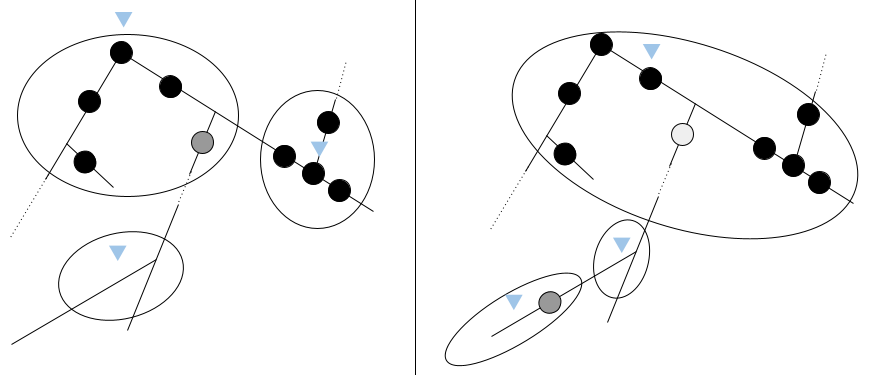
\includegraphics[width=0.7\textwidth]{Images/Deviation.png}
    \caption{Πιθανή κερδοφόρα αλλαγή}
    \label{fig:profDev}
\end{figure}
\end{proof}\


\section{Ανοιχτά προβλήματα}

Στις παραπάνω ενότητες είδαμε τα βασικά αποτελέσματα για το πρόβλημα χωροθέτησης υπηρεσιών αλλά και από που πηγάζει η δυσκολία του προβλήματος. Επιπλέον, είδαμε πως αν εστιάσουμε στα ``πραγματικά" στιγμιότυπα, από τη σκοπιά της ανάλυσης των αλγορίθμων πέρα της χειρότερης περίπτωσης, μπορούμε σχεδιάσουμε καλύτερους αλγορίθμους για προβλήματα που είναι πολύ δύσκολα στη γενική περίπτωση.Στον \textsc{Optimal} μηχανισμό είδαμε ότι πρέπει να αποκλείσουμε τα στιγμιότυπα που περιέχουν singleton clusters διότι ένας παίκτης μπορεί να δηλώσει μια θέση πολύ μακριά για να κερδίσει. Για να αντιμετωπίσουμε αυτό το πρόβλημα μια ενδιαφέρουσα ιδέα είναι να περιορίσουμε το εύρος των πιθανών τοποθεσιών που μπορεί να δηλώσει κάθε παίκτης σε σχέση με τη πραγματική του τοποθεσία. Σε αυτή τη περίπτωση πρέπει να δούμε πόσο ευσταθές πρέπει να είναι το στιγμιότυπο ώστε η βέλτιστη λύση να είναι φιλαλήθης. Μια άλλη κατεύθυνση είναι να ``χαλαρώσουμε" τον ορισμό της ευστάθειας σε ένα που είναι πιο πιθανό να περιγράφει τα πραγματικά στιγμιότυπα. Έχει προταθεί στη βιβλιογραφία για το clustering τα $(\g,\epsilon)$-ευσταθή στιγμιότυπα, στα οποία  για κάθε γ-διαταραχή το πολύ ένα μικρό ποσοστό $\epsilon$ σημείων αλλάζουν cluster.

\begin{english}

\chapter{Introduction}
``How can a group of individuals choose a winning outcome from a given set of options?" This is a question that has been studied in various fields like sociology (social choice theory), economics (game theory), and most recently, computer science (algorithmic game theory and computation social choice). Throughout this thesis, we will focus on the algorithmic aspect of the previous question and, specifically, on how we can effectively achieve a desirable outcome. These types of problems are studied in the field of \textit{Algorithmic Mechanism Design}, an intersection between \textit{Economic Theory} and \textit{Computer Science}. In classic mechanism design, the goal is to design a system for multi-participant environments. Depending on the setting, we are interested in different performance objectives like revenue maximization and social welfare maximization. Since the agents are strategic and rational, the system needs to ensure that all the agents will behave as the designer intended. Algorithmic mechanism design also considers computational constraints. Using tools from theoretical computer science while respecting game-theoretic constraints, the goal is to design efficient mechanisms.


%The prototypical problem in mechanism design is to design a system for multiple self-interested participants, such that the participants' self-interested actions at equilibrium lead to good system performance. Typical objectives studied


%Algorithmic game theory, as the name suggests, is an area in the intersection of game theory and computer science, with the objective of understanding and design of algorithms in strategic environments. We can see Algorithmic Game Theory from two perspectives: \textbf{\textit{Analysis:}} given a game with a predefined set of rules the goal is to analyze the outcome based on the behavior of the strategic agents (e.g., calculate and prove properties on their Nash equilibrium or compute the price of anarchy) \textbf{\textit{Design:}} design games that have both good game-theoretical properties, such as truthfulness and socially desirable outcome, and algorithmic properties, namely computational efficiency. This area is called ``\textit{algorithmic mechanism design.}"


\section{Motivation}

The \emph{Facility Location Problem} is one of the most fundamental and well-studied problems in Theoretical Computer Science, Operation Research, and recently Algorithmic Mechanism Design. Such problems are motivated by natural scenarios in Social Choice, where the government plans to build a fixed number of public facilities in an area like schools, libraries, or hospitals(e.g., see \cite{Miyagawa}). Apart from locating actual facilities, the problem has a wide range of applications, including non-geographic problems such as selecting a committee to represent people with differing political views. 


Let us look at it as an optimization problem first. The goal is to find the optimal placement of facilities to minimize transportation costs given a set of locations in a metric space. However, there are many applications where the locations are not publicly known and have to be reported by strategic agents. Now the goal is to design a strategyproof mechanism, i.e., does not incentivize agents to lie, which is also efficient with respect to the optimal solution. In many settings in Mechanism Design (e.g., auctions), payments guarantee that the optimal solution is strategyproof. On the other hand, payments could be illegal or unethical in Social Choice environments, such as Facility Location games\cite{SV07}. Procaccia and Tennenholtz \cite{Procaccia2013} showed that strategyproofness could also be achieved without payments by sacrificing the solution's optimality, thus initiating the research on \emph{Approximate Mechanism design without Money}.

Since then, the problem has been studied in many different settings and generalizations. There are two survey papers to get a complete overview of the problem: one for mechanism design for Facility Location Problems \cite{Chan2021} and one for approximation algorithms for Facility Location and Clustering Problems \cite{An2017}. In this thesis, we are going to focus on the mechanism design aspect of the problem. This problem has been studied for different metric spaces. One of the most researched setting is the $k$-Facility Location on the line (\cite{Fotakis2014,Fotakis2013sp,GolombT17,Lu2009,Nissim2010}).  It is also been researched for restricted metric spaces more general that the line(e.g., trees, circles, and plane \cite{Alon2010,Dokow2012,Filimonov2021,Goel2020,Meir2019}) and general metric spaces (\cite{Fotakis2013, Lu2010}). Another direction is to design mechanism for different objective functions, like \emph{maximum cost} \cite{Procaccia2013,Fotakis2013sp} and \emph{mini-sum-of-squares}\cite{Feldman2011}. For all those variations we assume that all the facilities are homogeneous. Recently, there is some work where the facilities serve different purposes (\cite{Li2021,Kyropoulou2019,Serafino2016}). There are also considered not single-peaked preference profiles   (\cite{MeiLYZ19,CHEN2020185,Feigenbaum2020})



In this thesis, we are going to focus on the classic $k$-Facility Location games, where $k$ uncapacitated facilities are placed in a metric space based on the preferences of $n$ strategic agents. Our goal is to minimize the social cost objective, namely the sum of the distances from each agent to the nearest facility. When the agents are located on the real line, we have a complete characterization of deterministic strategyproof mechanisms. For one facility, the mechanism that places the facility at the median location is strategyproof and optimal with respect to the social cost \cite{Procaccia2013}. For two facilities, the only strategyproof mechanism that exist places the facility at the leftmost and the rightmost locations (\textsc{Two Extremes} mechanism) and has an approximation ratio at most $n-2$ \cite{Procaccia2013,Fotakis2014}. However, for three or more facilities, there is no deterministic anonymous strategyproof mechanisms for k-Facility Location with a bounded approximation ratio \cite{Fotakis2014}. On the positive side, randomized mechanism achieve better approximation ratios. For 2-Facility Location games \textsc{Proportional Mechanism} achieves a constant approximation ratio of 4 \cite{Lu2010}. The \textsc{Inversely Proportional Mechanism} \cite{escoffier2011} has $n/2$-approximation ratio for $k$-facility location games with $n=k+1$ agents. Fotakis and Tzamos \cite{Fotakis2013sp} proposed the \textsc{Equal Cost} a randomized strategyproof mechanism with an approximation ration at most $n$ for any number of agents.

\begin{table}[ht]
    \centering
    \begin{tabular}{|c|c|c|c|}
         \hline
         & $k=1$ & $k=2$ & $k\ge3$ \\ \hline 
        Deterministic & 1\cite{Moulin1980} & $n-2$ \cite{Procaccia2013} & $\infty$ \cite{Fotakis2013}\\ \hline
        Randomized & 1\cite{Moulin1980} & 4 \cite{Lu2010} & $n$ \cite{Fotakis2013sp} \\ \hline
    \end{tabular}
    \caption{Best known results of approximation ratio for $k$-Facility Location on the line}
    \label{tab:summaryLine}
\end{table}


When the agents are located on more general metric spaces than the line, the problem becomes much more complicated. For tree metrics, for one facility the mechanism that places the facility at the median location is strategyproof and optimal \cite{Schummer2002}, but for two or more facilities there is no deterministic strategyproof mechanism with a bounded approximation. When the agents are located in a circle then any strategyproof mechanism is a dictatorship.

%+++++ extra power to the mechanism imposing mechanism and verification.

We can overcome the difficulty of the problem by giving ``additional power" to the mechanisms. Nissim, Smorodinsky, and Tennenholtz first proposed the class of \emph{imposing mechanisms} \cite{Nissim2010}. In that class, the mechanism can restrict the way agents are allowed to exploit the outcome. In the Facility Location setting, for example, agents are forced to connect to the facility closest to their reported location, even if there is a facility closer to their true location. This way, an agent that misreports has a greater connection cost since she cannot select the facility closest to her ideal location. Using the same techniques, Fotakis and Tzamos \cite{Fotakis2013} showed that the Winner Imposing version of the Proportional mechanism for the $k$-Facility Location is strategyproof and has an approximation ratio of at most $4k$. The mechanism requires that any agent that has a facility at her reported location connect to it. 

Another way to ensure strategyproofness and better approximation ratios is to consider \emph{mechanisms with local verification}. This was first introduced by Green and Laffont \cite{Green1986}. In order to model partial verification, they restricted the set of each agent’s allowable deviations to a so-called correspondence set. Later, Nisan \cite{Nisan2001} proposed a mechanism with verification for scheduling problems in unrelated machines, where each machine is controlled as a selfish agent. The mechanism has two stages: first, in the declaration phase, the agents report their types(namely the time of execution for each job) and the mechanism returns an allocation; then, in the execution phase, each machine executes the tasks it is allocated. The payments are given after the execution, so the mechanism can verify if the agents reported their true types and punish those who lied by reducing their payments. This notion of local verification has been adapted for different settings, see for example \cite{Auletta2009,Carroll2012,Caragiannis2012,Archer2014,Fotakis2015,Fotakis2016}.


Note that in the class of imposing mechanisms, the mechanism does not know whether or not an agent lied, but the way it restricts any agent's post-action options ensures that any lying agent will be penalized. On the other hand, a mechanism with verification can identify agents that lied and punish them. 


%We underline that liars still get utility from the selected outcome. It just happens that their preferences are not taken into account in the allocation. For these reasons, the penalty of exclusion from the mechanism is mild and compatible with the spirit of mechanisms without money

\section{Beyond Worst Case Analysis}

The previous results are based on the worst-case analysis framework in which an algorithm is characterized by its performance on the worst possible input. A good worst-case guarantee shows that an algorithm works well without any assumptions. However, in many interesting problems, this is impossible. To get better insight about an algorithms performance we want to move beyond the worst-case \cite{Rough20}. 

Take the problem of linear programming, where the goal is to minimize (or maximize) a linear objective function subject to linear constraints. Two algorithms solve this problem: the simplex method (exponential time in the worst-case) and the ellipsoid method (polynomial in the worst-case). Yet, empirically, simplex performs way better than the ellipsoid method. 

In this work we are going to focus on $\emph{Perturbation Stability}$. The notion of perturbation stability was first introduced by Bilu and Linial \cite{Bilu2009} for the Max-Cut Problem. Intuitively stability implies that small perturbation on the input does not change the optimal solution. By restricting our attention to stable instances, that model ``real world" instances, we can find the optimal solution. This was later adapted for clustering problems \cite{Balcan2011, Awasthi2012, Balcan2015, Angelidakis2017,Agarwal2020}. Clustering is the task of grouping a set of points in such a way that objects in the same group are more similar (in some sense) to each other than to those in other groups. Clustering, as an optimization problem, is $NP$-hard for most commonly used objective functions (e.g, $k$-median\cite{Mahajan2012}, $k$-center). However, simple clustering algorithms perform well in practice because the clusters are well defined. The notion of stability captures the structure that is usually found in practical instances. Therefore, by restricting our domain to a subset of instances, namely perturbation stable instances, we can design exact algorithms for an $NP$-hard problem.


%{-θέλει αλλαγή-}
We will call a clustering instance $\g$-\emph{perturbation stable} if the optimal clustering remains the same even if we scale down any subset of the entries of the distance matrix by a factor of at most $\g$. By focusing on the geometry of the instance, we show that in stable instances, all the inter-cluster distances are bounded by some intra-cluster distance. We will show three properties that hold in any $\g$-stable instance: \emph{Center-Proximity} (Definition \ref{Cprox}), \emph{Weak Center-Proximity} (Lemma \ref{WCprox}) and \emph{Cluster Separation Property} (Lemma \ref{CSprop}). 

\section{Facility Location on Stable instances and Contribution}



Since clustering and Facility Location games are closely related problems, an interesting question is whether we can achieve better results using the ideas and techniques from perturbation stability. The main difficulty in both problems is identifying the optimal clusters, namely the groups of points or agents that are served by the same center or facility. However, in Facility Location games, the agents are strategic, which means even if only one agent misreports her ideal location, the new instance can have a very different clustering structure than the original. Therefore, the question actually is how much power an agent has in manipulating the output of a mechanism assuming stability of the instance and, consequently, well-defined clusters.





 Fotakis and Patsilinakos \cite{Fotakis2021} initiate the study in that direction. The main idea is that the class of instances that appear in the real world are stable, and therefore, the mechanism should perform well only in those instances. Therefore, they consider the $k$-Facility Location games on the line restricted on perturbation stable instance. They showed that the optimal solution is strategyproof for $(2+\sqrt{3})$-stable instance, if the optimal clustering does not include  any singleton clusters. Let us point out that without any assumptions about the input, the optimal solution is not strategyproof, even for 2-Facility location games on the line. To avoid the restriction on stable instances with out singleton clusters the also proposed a randomized strategyproof mechanism with a constant approximation ratio for $5$-stable instances. Moreover, focusing on stable instances does not make the problem trivial. Extending the impossibility result for $k$-Facility Location games with $k\ge3$, they also proved that there is no deterministic anonymous strategyproof mechanism for $k$-Facility Location, with $k\ge3$, on $(2-\delta)$-stable instances with bounded approximation ratio for any $\delta>0$.

Our goal in this theses is to see how we can extend the previous results into more general metric spaces than the line. In the unrestricted domain the problem becomes non-trivial even when we want to place one in a circle or two facilities in a tree. We show that the optimal solution is strategyproof for $k$-Facility Location for $2+\sqrt{3}$ in tree metrics.




\chapter{Mechanisms for Facility Location games}
%\section{Facility Location}

In this chapter, we will present the main results of the Facility Location Problem in more detail. To better understand the problem, we will start with some useful definitions from the relevant field of Social Choice. Then we will formally define the setting and the basic concepts of \emph{Algorithmic Mechanism Design}.

\section{Social Choice and Single Peaked Preferences}

Social choice theory is the study of collective decision processes and procedures. How can a group of individuals choose a winning outcome (e.g., policy, electoral candidate) from a given set of options? In the most general setting there is a set $N$ of $n$ agents and a set $\A$ of alternatives. Each agent has a private order of the alternatives $\succ_i$ over the alternatives in $\A$. Let $L$ be the set of all linear orders of $\A$. A \emph{social choice function} $f:L^n \rightarrow \A$ maps the agents' preferences to a single alternative. A social choice function must satisfy the following properties:
\begin{definition}[Unanimous]
A social choice function $f$ is unanimous if, when all player prefer a certain outcome more than anything else, then that outcome must be the alternative chosen by the mechanism. That is, if $\exists a \in\A$ such that $\forall b\in\A$ and $i \in  N$, $a \succ_i b$ then $f(\succ_1,...,\succ_n) =a$.
\end{definition}
\begin{definition}[Onto]
 A social choice function $f$ is onto if any alternative can be reached given the appropriate preference profiles That is, $\forall a \in\A$, $\exists \x\in L^n$ such that $f(\x) = a$.
\end{definition}
\begin{definition}[Pareto Optimal]
 A social choice function $f$ is Pareto optimal if no other alternative is more preferred by every agent than the alternative chosen by the mechanism. That is, if $f(\x)=a$ for a $\x\in L^n$, then $\nexists b\in\A$ such that $b\succ_i$, $\forall i \in N$.
\end{definition}
\begin{definition}[Strategyproof]
A social choice function $f$ is strategyproof if no agent can change the outcome to a more preferable by misreporting her preferences. That is, for all preference profiles $\succ_1,...,\succ_n$ and any agent $i$, and any alternative preference $\succ_i'$: $f(\succ_1,...,\succ_i,...,\succ_n) \succ_i f(\succ_1,...,\succ_i',...,\succ_n)$.
\end{definition}

Our goal is to find the best possible outcome given the agents' preferences. The first three properties ensure that the selected outcome is efficient, namely desirable for all the agents. The agents, on the other hand, are selfish and strategic, aiming to maximize their utility. This is why, if we want the social function to be fair, the fourth property is crucial.

An other important property of social choice function is \emph{anonymity}, namely that the selection is based on the preference profiles only and not on the agent reporting it. This implies that all agents count the same in decision making.
\begin{definition}[Anonymous]
A social choice $f$ is anonymous if for all permutations $\pi$ and all profiles $(\succ_1,...,\succ_n)\in L^n$: $f(\succ_1,...,\succ_n) =f(\succ_{\pi(1)},...,\succ_{\pi(n)})$ 
\end{definition}

There are social choice functions that do not satisfy anonymity. For example, a \emph{dictatorial} social choice function that always selects the most preferred alternative for a particular agent, ignoring the preference profiles of the rest of the agents. We will call this agent a dictator. A dictatorial social choice function is strategyproof and Pareto optimal, but not fair because not all agents count the same.


\begin{definition}[Dictator]
An agent $i$ is a dictator in a social choice function $f$ if for all $\succ_1,...,\succ_n\in L$: $f(\succ_1,...,\succ_n)=a$ where $a\succ_i b, \forall b\in \A$ with $b\ne a$.
\end{definition}



A simple and intuitive example of a social choice function is the majority vote. If there are only two alternatives then the majority is strategyproof. If there are $3$ or more alternatives, however, the majority is not strategyproof. An agent may change her preference profile to prevent her least liked option from being selected. Unfortunately, there is an impossibility result that states we cannot do anything better than a dictatorship when there are more that 3 alternatives. 



\begin{theorem}[Gibbard \cite{Gibbard1973} - Satterthwaite \cite{Satterthwaite1975}]
Let $f$ be an incentive compatible
social choice function onto $\A$, where $\A \ge 3$, then $f$ is a dictatorship.
\end{theorem} 

One way to overcome the impossibility result of the previous theorem is to introduce payments into the model. There are many strategyproof mechanisms with money. The idea is that if an agent misreports in an attempt to benefit, the extra payment from the mechanism will be more than the actual decrease in the cost. However, as we mentioned before, we are interested in applications where payments are not an option. So, in order to overcome the impossibility result without money, we are going to restrict the domain of possible preference profiles to single-peaked preferences. Preferences are said to be single-peaked if the alternatives can be represented as points on a line, and each agent has a unique most preferred point (``"peak" preference) and points that are further from her peak are preferred less. It is natural to assume that the agents have single-peaked preferences for many problems. For example, in the Facility Location setting, where the government wants to place public facilities, any agent would prefer the facility closest to her ideal location since any other facility will only increase the transportation cost.


\begin{definition}[Single-Peaked Preferences]
Preferences are said to be single-peaked if the alternatives can be represented as points on a line, and there exists an alternative $a \in \A$ (the peak) such that if $x<y<a \implies y \succ x$ and if  $a<x<y \implies x\succ y$. 
\end{definition}

Moulin \cite{Moulin1980} showed that if all the agents have single-peaked preferences, there exists a strategy-proof mechanism that only depends on the peak of each agent.


\begin{theorem}
Assuming single peakedness, a rule $f$ is strategyproof, onto and anonymous if and only if there exists $a_1,a_2,...,a_n\in [0,1]$ such that for all peaks $(x_1,...,x_n)\in \mathbb{R}$.
\end{theorem}




\section{Preliminaries for Facility Location Games}

By the definition of single-peaked preferences we can see that a profile is single-peaked if for any two points on the same side of the peak the agent always prefers the one which is closer to her peak. But there is no way to now by ``how much" agent $i$ prefers alternative $x$ over $y$. From now on, we are going to assume that the agents rank the all the alternative locations based on the distance from their peak.


\begin{definition}[Facility Location]
Let $N= \{1,..,n\}$ be a set of agents. The agents are located in a metric space $(X,d)$, where $d:X \times X \rightarrow  \mathbb R_{\ge 0} $ is the distance function. The function $d$ is a metric on $X$ satisfying $d(x,x)=0$ for all $x\in X$, $d(x,y)=d(y,x)$ for all $x,y\in X$ (\emph{symmetry}) and, $d(x,z)\le d(x,y)+d(x,z)$ for all $x,y,z\in X$ (\emph{triangle inequality}). Each agent $i\in N$ has a private location $x_i \in X$. We refer to the tuple $\x=(x_1,...x_n)$ as the \emph{location profile} or \emph{instance}.
\end{definition}


For a location profile $\x$ and an agent $i$, let $\x_{-i}$ denote the tuple $\x$ without the coordinate $x_i$. Similarly, for a non-empty set $S$ of indices, let $\x_S=(x_i)_{i\in S}$ be the locations of agents in $S$ and $\x_{-S}=(x_i)_{i\notin S}$ the tuple $\x$ without the location of agents in $S$.  

Each agent reports her ideal location to the mechanism $M$. A \emph{deterministic mechanism} $M$ for $k$-Facility Location maps an instance $\x$  to a $k$-tuple $\vec{c}=(c_1,...,c_k)\in X^k$. We let $M(\x)$ denote the outcome of $M$ in instance $\x$. Similarly, a \emph{randomized mechanism} $M$ maps an instance $\x$ to a probability distribution over $k$-tuples $(c_1,...,c_k)\in X^k$.

For a location profile $\x$ and a mechanism $M$, we define the \emph{connection cost} of agent $i$ as the minimum distance of her private location to the closest facility, $cost(x_i,M(\x)) = min_{1\le j \le k} \{d(x_i,c_j) \}$. The \emph{social cost} of a mechanism $M$ is the total distance of the agents' locations to the nearest facility, $cost(\x,M(\x)) = \sum_{i=1}^n d(x_i,M(\x))$. 
%The \emph{maximum cost} of $M$ is the maximum distance of an agent to her closest location, $MC(\x,M(\x)) =  max_{i\in N } \{ d(x_i,M(\x))\}$

Since each agent is strategic, it is easy to see that the goal of each agent is different from the mechanism's. The mechanism's objective is to minimize the social cost, but each strategic agent seeks to minimize its connection cost. This divergence between the two goals motivates an agent to manipulate the mechanism by reporting a false location to achieve a better connection cost. This is why strategyproofness is a crucial property that any mechanism should satisfy.

\begin{definition}[Strategyproof]
A mechanism is strategyproof if for all location profiles $\x$, any agent $i$, and all locations $y$: 
\[cost(x_i,M(x)) < cost(x_i, M(x_{-i},y))\]
\end{definition}

A mechanism can also be \emph{group strategyproof} if for any coalition misreporting their location simultaneously, at least one does not benefit. Formally: 
 
\begin{definition}[Group Strategyproof]
A mechanism is strategyproof if for location profiles $\x$, all coalitions $S \subset N$ and all location profiles $\xx = (\x_{-S},x_S')$, there exists an agent $i\in S$ such that
\[ cost(x_i,M(\x)) \le cost(x_i,M(\xx))\]
\end{definition}

\begin{definition}[Image Set]\label{imageSet}
For any mechanism $M$, the \emph{image set} of agent $i$ with respect to a location profile $\x_{-i}$ is the set of all the possible facility locations the agent can obtain by varying her reported location. Formally:
\[ I_i(\x_{-i}) = \{a \in  X: \exists \;y \in X \; with \; M(\x_{-i},y)\}\]
\end{definition}

We can see the image set as the power an agent has on the mechanism. Any strategyproof mechanism $M$ always outputs some location in $I_i(\x_{-i})$ that is closest to the reported location as shown in the following lemma.

\begin{lemma}\label{imageSetLemma}
Let $M$ be a strategyproof mechanism for the $k$-Facility game. For every location profile $\x \in X^n$ and any agent $i\in N$ we have:
\[ cost(y,M(\x_{-i},y)) = \inf_{a\in I_i(\x_{-i})} \{d(a,y)\}\]
\end{lemma}

\begin{proof}
For the location profile $\xx=(\x_{-i},y)$ let $a\in M(\xx)$. Assume for contradiction that exists $a^*\in I_i(\x_{-i})$ such that $d(a^*,y) < d(a,y)$. By the definition of the image set there exists a $y^*$ such that $a^* \in M(\x_{-i},y^*)$. Then, if agent $i$ is located at y she can benefit by misreporting to $y^*$ lowering her connection cost from $cost(y, M(\x_{-i},y))$ to $d(a^*,y)$. This contradicts the assumption that $M$ is strategyproof
\end{proof}

We can extend the previous definition of image set from a single agent to a group of agents. For a given mechanism $M$ we define the image set of agents in a subset $S$ with respect to a location profile $\x_{-S}$ as the set of all possible facility locations they can obtain by varying their reported location:

\[ I_S(\x_{-S}) = \{a \in X: \exists\;\vec{y} \in X^{|S|} \; with \; M(\x_{-S},\vec{y})\}\]

We can also extend the previous lemma to hold for partial group strategyproof mechanisms, when all agents in the coalition report the same location.
\begin{lemma}
Let $M$ be a strategyproof mechanism for the $k$-Facility Location game. For every location profile $\x \in X^n$, any non-empty set of agents $S\subset N$, $\vec{y}$ and $\vec{y}=(y,...,y)$ we have:
\[ cost(y,M(\x_{-S},\vec{y})) = \inf_{a\in I_S(\x_{-S})} \{d(a,y)\}\]
\end{lemma}


%\section{Facility Location}

%introo  single peak preference and distance function 

\section{Facility Location on the Line}

In this section, we are going to focus on \emph{Facility Location} on the real line. Let $N=\{1,...,n\}$ be the set of agents. Each agent has a private ideal location $x_i\in \mathbb{R}$. We can assume without loss of generality that the locations in the location profile $\x = (x_1, ..., x_n)$ are ordered ($x_1\le x_2\le...\le x_n$), since we focus on anonymous mechanisms. Given an instance $\x$ the most important locations are the leftmost and the rightmost because they delimit the instance. We denote the leftmost location as $lt(\vec{x})=min_{i\in N}\{x_i\}$ and the rightmost location as $rt(\vec{x})=max_{i\in N}\{x_i\}$. The distance function between any two locations is simply the length of the interval, $d(x,y) = |x-y|$. 
%{+??+}


%----------------------------------------------------------------------------
%One facility on the line
\subsection{Locating one facility}

We start with the simplest setting. Given an instance $\x$ we want to place one facility that achieves the best possible social cost in a strategyproof way. 

\begin{theorem}
The mechanism that selects the median location of the reported instance is strategyproof and optimal for the social cost objective.
\end{theorem}

\begin{proof}
We first show that the median location, $med(\vec{x})$, is the optimal solution. If $n$ is odd the median location is $x_{(n+1)/2}$, if $n$ is even any location in the interval $[x_{n/2},x_{n/2+1}]$ is optimal without lost of generality we consider $x_{n/2}$ to be the selected location. Suppose the facility is placed at a location to the left of the median location, let that location be $x$. Then, at least half of the agents' connection cost has increased by $d(x,med(\vec{x}))$, and at most half of the agents' connection cost has decreased by $d(x,med(\vec{x}))$. This makes the social cost of $x$ higher than the optimal. The same holds for any location selected to the right of the median.

We now show that the mechanism is strategyproof. The agent located at $med(\vec{x})$ has no initiative to misreport her location, since her connection cost is zero. Suppose an agent $i$ located at $x_i$ misreports to $x_i'$. Without loss of generality we can assume that $x_i<med(\vec{x})$. If $x_i'<med(\vec{x})$ then the output of the mechanism does not change. If $x_i'>med(\vec{x})$ the median location moves to the right leading to an increase in her cost.
\end{proof}



%------------------------------------------------------------
%Two Facilities on the Line

\subsection{Locating two facilities}
This section extends the previous setting from locating one facility on the real line to locating two. Now a mechanism returns a 2-tuple $\vec{c}=(c_1,c_2)$ with the location of the facilities; we can assume that $c_1 \le c_2$. Each agent connects to the nearest facility with connection cost equal to $cost(x,\vec{c})=min\{ d(x,c_1), d(x,c_2)\}$. 


Let us focus on the optimization problem of locating the two facilities without considering the strategic agents' motives. Let $\vec{x}$ a location profile, and $c_1$,$c_2$ the optimal facility locations.  We can split the agents into two (non-empty) groups based on which facility they prefer. The agents that prefer $c_1$ belong to the "left" set $L(\vec{x})$, and the rest belong to the "right" set $R(\vec{x})$. Using the same argument as in the previous setting for one facility on the line, given the sets $L(\vec{x})$ and $R(\vec{x})$, the optimal locations $c_1$ and $c_2$ are the median of each set. So, for an arbitrary location profile $\vec{x}$, we can compute the optimal solution by selecting the locations that minimize the social cost over the (n-1) choices for $L(\vec{x})$ and $R(\vec{x})$.

%%%????????????????????????
Unfortunately, the mechanism that selects the optimal solution is not strategyproof. The reason is that the sets in the optimal solution are susceptible to minor changes, and the agents can benefit from that. In order to design a strategyproof mechanism we need to extract $L(\vec{x})$ and $R(\vec{x})$ in a strategyproof way. Since both sets are non-empty we are sure that the leftmost agent belongs to $L(\vec{x})$ and the rightmost agent to $R(\vec{x})$. So the mechanism that places the facilities to the leftmost and the rightmost agent is strategyproof and achieves $(n-2)$-approximation ratio. As we will see bellow this is the only deterministic anonymous strategyproof mechanism with bounded approximation for the $2$-Facility Location game. 

\begin{theorem}
The \textsc{Two Extremes} mechanism that places the facilities at the leftmost $lt(\vec{x})$ and the rightmost $rt(\vec{x})$ is a $(n-2)$-strategyproof mechanism for social cost.
\end{theorem}
\begin{proof}
To show the approximation ratio consider the location profile with $n$ agents, where one agent is located at 0, $n-2$ agents are located at $\epsilon>0$ (arbitrarily close to 0), and one agent at 1. The optimal solution places one facility at $\epsilon$ and the other at $1$. The social cost of the optimal solution is $SC^* = \epsilon$. The social cost of the solution outputted by the mechanism is $(n-2)\epsilon = (n-2) SC^*$, since $(n-2)$ agents have connection cost equal to $\epsilon$.

We now show that the mechanism is also strategyproof. Let $\vec{x}$ be a location profile. Any agent reporting a location in the interval $[lt(\vec{x}),rt(\vec{x})]$ cannot change the output of the mechanism. However, if an agent reports a location $x' \in (-\infty,lt(\vec{x})) \cup (rt(\vec{x}),\infty)$ will move the facility further away from her ideal location. So, no agent can benefit by misreporting her location
\end{proof}



%-------------------------------------------------------------------------

In the paper \cite{Procaccia2013} Procaccia and Tennenholtz proved that any deterministic strategy proof mechmanism for 2-Facility Location game has approximation ratio of at least $1.5$. This result was later improved to $2$ \cite{Lu2009}, and then to $(n-1)/2$ \cite{Lu2010} . Fotakis and Tzamos \cite{Fotakis2014} proved a tight lower bound of $n-2$. From the latest result we conclude that the \textsc{Two Extremes} mechanism is the only deterministic, anonymous, strategy-proof mechanism with a bounded approximation ratio.  


The takeaway from the previous section is that we cannot improve the linear approximation ratio for any deterministic strategyproof mechanism. So, the next question is if we can achieve better results with randomized mechanisms. Fortunately, the answer is yes. The \emph{Proportional Mechanism} \cite{Lu2010} is strategyproof and achieves a constant approximation ratio. The idea for this mechanism is very simple and intuitive. Place the first facility uniformly at random among all the reported locations and the second with a probability proportional to its distance from the first. However, is not that simple to prove that the mechanism is indeed strategyproof with constant approximation ratio.

\begin{definition}[Proportional Mechanism]

Given a location profile $\vec{x}=(x_1,...x_n)$, the location of the two facilities are decided by the following random process:
\begin{itemize}
    \item\textbf{Round 1:} Choose agent $i$ uniformly at random from $N$. The first facility $c_1$ is placed at $x_i$

    \item\textbf{Round 2:} Let $d_j = d(c_1,x_j)$ be the distance from agent $j$ to the first facility. Choose agent $j$ with probability $\frac{d_j}{\sum_{k\in N}d_k}$. The second facility is placed at $x_j$.

\end{itemize}
\end{definition}




\begin{theorem}
The proportional mechanism for the two-Facility Location game is strategyproof.
\end{theorem}
\begin{proof}
Let $cost_k(x_i,M(\x))$ denote the expected cost of agent $i$ when the mechanism places the first facility facility on $x_k$. The agent that has a facility at her location experiences after the first round zero cost, so $cost_k(x_k,M(\x))=0$. Since the first facility is selected uniformly at random, we have that for any agent $i$ her total cost is:
\[ cost(x_i,M(\x)) = \frac{1}{n}\sum_{k=1}^{n} cost_k(x_i,M(\x)) = \frac{1}{n}\sum_{k\ne i} cost_k(x_i,M(\x)) \]



Let $\xx=(\x_{i},x_i')$ be the location profile after the deviation of agent $i$. We need to show that she cannot decrease her cost by misreporting her location. We need to show that for all $k\ne i$:

\[ cost(x_i,M(x)) < cost(x_i, M(\xx))\]

Fix the first facility on $x_k$. The expected cost of agent $i$ to the second facility, conditional on the first facility is at $x_k$, is:
\[ cost(c_2,x_i) = \sum_{j=1}^{n} { Pr[c_2=x_j]\cdot d(x_i,x_j)} = \sum_{j=1}^{n} { \frac{d_j}{\sum_{k=1 }^{n}d_k} d(x_i,x_j)}  = \frac{ \sum_{j=1}^{n}d_j \cdot d(x_i,x_j)}{\sum_{j=1}^{n}d_j} \]

Then we have that the cost of agent $i$ is the minimum between the distance to $x_k$ and the expected distance to the second facility:

\begin{align*}
   cost_k(x_i,M(\x)) &= \min\bigg\{d_i, \frac{ \sum_{j=1}^{n}d_j \cdot d(x_i,x_j)}{\sum_{j=1}^{n}d_j}  \bigg\}\\
   &= \frac{\sum_{j=1}^{n}d_j \min\{d_i,d(x_i,x_j)\}}{\sum_{j=1 }^{n}d_j}\\
   &= \frac{\sum_{j\neq i}d_j \min\{d_i,d(x_i,x_j)\}}{\sum_{j=1 }^{n}d_j}
\end{align*}

Let $d_i'=d(c_1,x_i')$. The cost of agent $i$ if she misreports is:
\[ cost_k(x_i,M(\xx)) =\frac{\sum_{j\neq i}d_j \min\{d_i,d(x_i,x_j)\}}{\sum_{j=1 }^{n}d_j + (d_i'-d_i)} + \frac{d_i' \min\{d_i,d(x_i,x_i')\}}{\sum_{j=1 }^{n}d_j + (d_i'-d_i)} \]

We can get the following relation between $cost_k(x_i,M(\x))$ and $cost_k(x_i,M(\xx))$:

\begin{equation}\label{compCost}
cost_k(x_i,M(\xx)) =\frac{ cost_k(x_i,M(\x)) \sum_{j=1}^{n}d_j }{\sum_{j=1 }^{n}d_j + (d_i'-d_i)} + \frac{d_i' \min\{d_i,d(x_i,x_i')\}}{\sum_{j=1 }^{n}d_j + (d_i'-d_i)}    
\end{equation}


We need to distinguish two cases:
\begin{enumerate}[(i)]
    \item $d_i' \le d_i$: we have that $cost_k(x_i,M(\x)) < cost_k(x_i,M(\xx))$ because $\frac{\sum_{j=1}^{n}d_j }{\sum_{j=1 }^{n}d_j + (d_i'-d_i) }>1$ and the second term in the previous equality is non-negative.
    \item $d_i' > d_i$: This case is not that simple. If we subtract $cost_k(x_i,M(\x))$ from (\ref{compCost}), we have:
\[ cost_k(x_i,M(\xx)) - cost_k(x_i,M(\x)) =\frac{ -(d_i'-d_i)cost_k(x_i,M(\x))  }{\sum_{j=1 }^{n}d_j + (d_i'-d_i)} + \frac{d_i' \min\{d_i,d(x_i,x_i')\}}{\sum_{j=1 }^{n}d_j + (d_i'-d_i)}\]

So it suffice to show that:
\begin{equation}\label{s}
   d_i' \min\{d_i,d(x_i,x_i')\}-(d_i'-d_i)cost_k(x_i,M(\x)) \ge 0 
\end{equation}

We need to show that (\ref{s}) holds for both cases:
    \begin{enumerate}
        \item If $\min\{d_i,d(x_i,x_i')\} = d_i$. We have that $d_i \ge cost(x_i,M(\x))$ because agent $i$ always selects the facility closest to her location which cannot be further than the facility placed ad $x_k$. We also have $d_i' \ge d_i' - d_i$. By multiplying the previous inequalities we have that (\ref{s}) holds.
        \item If $\min\{d_i,d(x_i,x_i')\} = d(x_i,x_i')$. We have that $d_i'=d_i \ge cost(x_i,M(\x))$. From triangle inequality we have $d(x_i,x_i') \ge d_i'-d_i$. Again by multiplying the previous inequalities we get that (\ref{s}) holds.
    \end{enumerate}
\end{enumerate}

\end{proof}

It is very interesting that an agent cannot gain even if she knows where the first facility is placed after the first round.

\begin{theorem}
The approximation ratio of the Proportional mechanism for the two Facility Location game is 4 for any metric space.
\end{theorem}

The proportional mechanism is the best know randomized strategyproof mechanism for 2-Facility Location game. The previous know result \cite{Lu2009} has an approximation ratio of $n/2$. A a constant upper bound is a great improvement to the previous liner bound, but there is still a big gap between the upper bound and the only know lower bound for randomized mechanisms, which is $1.045$\cite{Lu2009}. 




\subsection{Locating more than two facilities}

As we previously saw the problem becomes significantly more difficult when we want to locate two facilities instead of one. For the 2-Facility Location games we saw that \textsc{Two Extremes} is the only deterministic and it has a linear approximation ration. Therefore, we cannot expect any better results for $k$-facility location games, when $k\ge3$. In fact we have a very negative result: there is no deterministic anonymous strategyproof mechanism with bounded approximation for $k\ge3$ \cite{Fotakis2014}. This holds even for $n=k+1$ agents. We are going to focus on the intuition behind the proof and present a sketch-proof.  We will refer to deterministic, anonymous, and strategyproof mechanisms with a bounded approximation ratio (in terms of $n$ and $k$) as \emph{nice mechanisms}.



The proof heavily relies at \emph{well-separated instances}, namely instances with $k-1$ isolated agents and two nearby agents. Let $\x = (x_1|x_2|...|x_k, x_{k+1})$ be a well separated instance. The optimal solution is to serve all the isolated agents by a different facility and the two nearby by from the remaining facility. First, we are going to show some properties of nice mechanisms. 

%Given a nice mechanism $M$ with an approximation ration $\rho$ ----- an $a$-approximation mechanism $M$  includes a pair of nearby agents at distance to each other less than $1/a$ times the distance between any other pair of consecutive agents. 


\begin{proposition}
Let $M$ be a nice mechanism for $k$-Facility Location on the line. For any $(k+1)$-location instance $\x$, $M_1(\x) \le x_2$ and $M_k(\x)\ge x_k$
\end{proposition}


\begin{proposition}
Let $M$ be a nice mechanism for $k$-Facility Location. For any $\x=(x_1|x_2|...|x_k,x_{k+1})$ well separated instance, $M_k(\x) \in [x_k,x_{k+1}]$
\end{proposition}

The following propositions show that in well-separated instances if a mechanism places a facility on the left of the nearby agents and we ``push" both agents to the right, while keeping the instance well-separated, the rightmost facility remains on the same agent. Similarly, if a mechanism places a facility on the right of the nearby agents and we ``push" both agents to the left then the rightmost facility remains on the same agent. 

\begin{proposition}
Let $M$ be a nice mechanism for $k$-Facility Location and let  $\x = (x_1|x_2|...|x_k,x_{k+1})$ be a well separated instance such that $M_k(\x) = x_k$. Then for every $\xx = (\x_{-\{k,k+1\}},x_k',x_{k+1}')$ well separated instance with $x_k \ge x_k'$ it holds $M_k(\xx) = x_k'$
\end{proposition}


\begin{proposition} \label{left}
Let $M$ be a nice mechanism for $k$-Facility Location and let  $\x = (x_1|x_2|...|x_k,x_{k+1})$ be a well separated instance such that $M_k(\x) = x_{k+1}$. Then for every $\xx = (\x_{-\{k,k+1\}},x_k',x_{k+1}')$ well separated instance with $x_{k+1} \le x_{k+1}'$ it holds $M_k(\xx) = x_{k+1}'$
\end{proposition}

Using the previous propositions we can show that any anonymous nice mechanism for $k$-facility location on $(k+1)$-agent instances always allocates facilities to the leftmost and to the rightmost agent.

\begin{lemma}\label{leftRight}
Let $M$ be a nice mechanism for $k$-Facility Location with $k\ge2$ and $n=k+1$. Then for all instances $\x=(x_1,...,x_{k+1})$ with $x_1\le...\le x_{k+1}$, $M_1(\x) = x_1$ and $M_k(\x)=x_{k+1}$.
\end{lemma}

We can now show that there is no nice mechanism for $k$-Facility Location when $k\ge3$.

\begin{theorem}
For every $k\ge3$, any deterministic strategyproof mechanism for $k$-Facility Location with $n\ge k+1$ agents on the line has an unbounded approximation ratio. 
\end{theorem}
The previous propositions and the lemma describe how any nice mechanism should ``behave". Suppose that there is a nice mechanism $M$ with a bounded approximation for 3-Facility Location. Let  $\x=(x_1|x_2|x_3,x_4)$ be a well-separated instance. By Lemma \ref{leftRight} $x_1$ and $x_4$ have a facility. And since the instance is well-separated agent $x_3$ is served by the facility at $x_4$. 
\begin{figure}[ht]
    \centering
    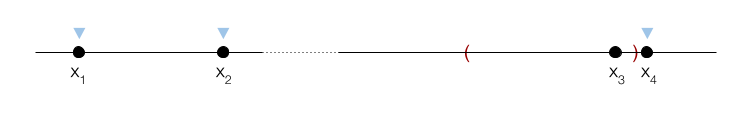
\includegraphics[width=12cm]{Images/imposibility1.png}
    \caption{$\x$}
    \label{fig:imp1}
\end{figure}

Let us remind the definition of the image set (Definition \ref{imageSet}). The image set of an agent $i$ is the set of facilities the agent can obtain by varying her reported location. Any interval in the complement of an image set $I_i(\x_{-i})$ is called a hole. By Lemma \ref{imageSetLemma} we have that the mechanism places a facility at the location in $I_i(\x_{-i})$ nearest to the location of agent $i$. Since agent $x_3$ is not allocated a facility in $\x$ there is a hole in the image set $I_3(\x_{-3})$ around $x_3$. Let $l$ and $r$ be the locations in $I_3(\x_{-3})$ nearest to $x_3$ on the left and on the right.(let the red lines represent the hole). Now consider the location profile $\y = (\x_{-3}, l+\epsilon)$. By Lemma \ref{imageSetLemma} the mechanisms should place a facility at $l$, since $l$ is the nearest location in the image set.


\begin{figure}[ht]
    \centering
    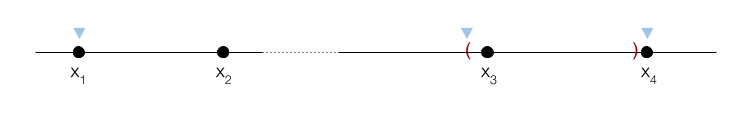
\includegraphics[width=12cm]{Images/imposibility2.png}
    \caption{$\y$}
    \label{fig:imp2}
\end{figure}

Now consider the location profile $\vec{z}=(\y_{-4},l)= (\x_{\{-3,4\}},\{l,l+\epsilon\})$. The mechanism is anonymous, which means we can rearrange the indices so that $x_1\le x_2 \le x_3\le x_4$. As a result, agents 3 and 4 switch indices in $\y$ and $\vec{z}$. We have that $M$ is strategyproof. Since in $\y$ and in $\vec{z}$ there is an agent at $l+\epsilon$ and in $\vec{z}$ an agent is moving closer to $l$, $M$ should keep a facility at $l$. By proposition \ref{left} we have that $x_4$ has a facility because $\x$ and $\vec{z}$ are well-separated instances and the nearby agents move to the right. But this way in $\vec{z}$ the nearby agents are allocated two facilities which makes the cost arbitrarily larger than the optimal.


%In $y$ and $z$ there is an agent at $l+\epsilon$. $M$ is strategyproof and since $M$ places a facility in $y$ at $l$ and in $z$ there is an agent at $l$, $M$ should keep a facility at $l$.
% In $\y$ and in $\vec{z}$ there is an agent at $l+\epsilon$ and in $\vec{z}$ an agent is moving closer to $l$. Since $M$ is strategyproof it should keep a facility at $l$


\begin{figure}[ht] 
    \centering
    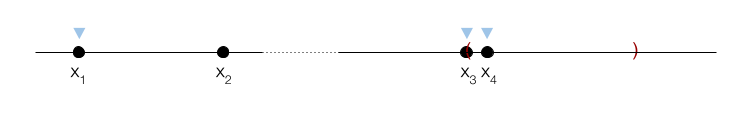
\includegraphics[width=12cm]{Images/imposibility3.png}
    \caption{$\vec{z}$}
    \label{fig:imp3}
\end{figure}



%---------------------------------------------------------------------------
% percentile mechanisms 
Even if we cannot have deterministic strategyproof mechanisms with a bounded approximation ration for the $k$-Facility Location games with $k\ge3$, there is a class of deterministic strategyproof mechanisms \cite{Sui2013}  for any $k\ge2$. A percentile mechanism splits the instance into $k$ parts, based on a predefined vector $\vec{p} \in (0,1)^k$, and allocates one facility at each part. One might think how can this class of mechanisms be practical if there is no guaranty for the outcome. However, in most ``real world" applications the designer has some knowledge of the preferences of the participating agents. This allows for empirical optimization of the vector $\vec{p}$. Let us formally define the percentile mechanisms.

\iffalse
\bigskip
Since we focus on anonymous mechanism we can assume without loss of generality that in an instance $\x = (x_1,...,x_n)$ all the agents' locations are in an ascending order ($x_1\le ... \le x_n$).  
\fi


\begin{definition}[$\vec{p}$-percentile mechanism]
The percentile mechanism is specified by a vector $\vec{p}=(p_1,...,p_k)$ where $0\le p_1\le...\le p_k \le 1$. The mechanism locates $j$th facility at the $p_j$th percentile of the reported locations. 
\[ c_j = x_{i_j}\; :\; i_j = \lfloor (n-1)\cdot p_j \rfloor +1 \]

\end{definition}

To better understand the mechanism let $\x = (x_1,...,x_9)$ be a location profile with $9$ agents. The $(0.25,0.75)$-percentile mechanism will place the first facility at $c_1=x_3$ since $\lfloor 8\cdot 0.25 \rfloor +1  = 3$ and the second facility at $c_2=x_7$ since $\lfloor 8\cdot 0.75 \rfloor +1 = 7$. 


\begin{figure}[ht]
    \centering
    
\includegraphics[width=12cm]{Images/percentile.png}
    \caption{Example of $(0.25,0.75)$-percentile mechanism for 9 agents}
    \label{fig:percentileExample}
\end{figure}

\begin{lemma}
The percentile mechanism is group strategyproof for any $\vec{p}$.
\end{lemma}

\begin{proof}
We are going to prove the lemma for $k=2$ but the proof is similar for $k\ge2$. Let $\vec{c}=(c_1,c_2)$ be the locations of the facilities when all the agents report their true preferences and $\vec{c}'=(c_1',c_2')$ be the locations after agents in a subset $S\subset N$ deviate from their true locations. Let $\Delta_1 = c_1-c_1'$ and $\Delta_2 = c_2'-c_2$. Now we need to show that at least one agent in $S$ does not benefit from the deviation. There are four cases to consider:
\begin{enumerate}[(i)]
    \item $\Delta_1\ge0$ and $\Delta_2>0$. That means that the first facility is moved to the left and the second to the right. In order for this to happen there is one agent that has an ideal location $x_i \in (c_1,c_2)$ who reported a location either to the left of $c_1$ or to the right of $c_2$. Otherwise the facilities could not move in such way. Now the cost of agent $i$ is:
    \begin{align*}
        cost(x_i,M(\xx)) &= min(d(x_i,c_1'),d(x_i,c_2'))\\
        &\ge min(d(x_i,c_1),d(x_i,c_2))\\
        &= cost(x_i,M(\x))
    \end{align*}
    \item $\Delta_1\ge0$ and $\Delta_2<0$. Now both facilities moved to the left. That means there is an agent $i$ with $x_i>c_2$, that reported a location to the left of $c_2$. Her cost is:
    \[ cost(x_i,M(\xx)) = x_i -c_2' \ge x_i-c_2 = cost(x_i,M(\x))\]
    \item $\Delta_1<0$ and $\Delta_2\ge0$. This case is completely symmetric to the previous case.
    \item $\Delta_1<0$ and $\Delta_2<0$. The first facility is moved to the right and the second to the left. As in the second case there is an agent to the right of $c_2$ that reported a location to the left. She cannot benefit from this deviation.
\end{enumerate}
Note that if $\Delta_1=0$ and $\Delta_2=0$ represents the case where neither facility moves and no agent benefits from the deviation. So without loss of generality we can assume that at least one of $\Delta_1$ or $\Delta_2$ is non-negative. 

\end{proof}
 
The main idea behind the proof is that the mechanism selects where to open a facility without ``looking" at the instance. Like in the example above in any instance (with $9$ agents) the $(0.25,0.75)$-percentile mechanism  will place the facilities at the $3$nd and $7$th agent respectively without looking at their actual locations. In order for an agent to change the outcome of the mechanism she would have to report a location $x'$ in a different part than her true preference. Like in the setting with one facility (and the median location) this deviation would move the facility further away making it a non profitable deviation. 


The \textsc{Two Extremes} mechanism mention above belongs in the class of percentile mechanism with a vector $\vec{p}=(0,1)$. It is also the only mechanism within the family of percentile mechanisms that has a bounded approximation ratio. For any $\vec{p}\neq (0,1)$ we can create an instance with arbitrarily small cost but since the mechanisms does not ``look" at the instance the solution will have arbitrarily large cost. Consider a location profile $\x=(0,\epsilon,1)$ where $\epsilon>0$ but arbitrarily close to $0$. The $(0,0.6)$- percentile mechanism will allocate the facilities to the first two agents. It is easy to see that the cost of the optimal solution is $\epsilon$ but the cost of the solution of the mechanism is $1-\epsilon$. Thus, the approximation ratio is unbounded.

~\\\textbf{Randomized mechanisms}

%{+Counter-example for proportional for 3 facilities+}
Again we may get better results if we consider randomized mechanism for $k$-Facility Location on the line. Unfortunately, a simple extensions of the proportional mechanism is not strategyproof even when $k=3$. The first two facilities are allocated like in the Proportional mechanism and the third is placed on a location of an agent with probability proportional to her minimal distance to the first two facilities. 

Consider this counter-example: there exist $n_0$ agents at $0$, $n_1$ agents at location $1$, $n_2$ agents at location $1+x$ and 1 agent at location $1+x+y$. Here $n_0$ is sufficiently large such that we can assume the first facility to be always located at $0$. In this configuration, let $y=100$, $x=10^{100}$, $n_1=50$ and $n_2=4$. An agent at location 1 may have the incentive to misreport to location 1+x. 

If we take a closer look at the instance, we can see that the distance between locations 0 and 1 is 1, and between locations $1+x$ and $1+x+y$ is $y$. By selecting $x=10^{100}$, the distance between locations 1 and $1+x$ is huge compared to the other two distances. By construction, the mechanism places the first facility at 0. Since the second facility is placed with a probability proportional to the distance to the first facility, the agent's deviation to $1+x$ increases the probability the second facility is placed at $1+x$. But that also means that the third facility  has an increased probability of being placed  at her true location, making that mechanism manipulable.




%{+Imposing mechanisms+}
Due to the negative results in the general setting new approaches were proposed. Imposing mechanisms was proposed by Nissim, Smorodinsky, and Tennenholtz \cite{Nissim2010}, namely mechanisms able to restrict how agents exploit their outcome. Fotakis and Tzamos \cite{Fotakis2013} showed that the winner-imposing version of the Proportional mechanism is strategyproof for the $k$-Facility Location game, and achieves an approximation ratio of at most $4k$. In this setting any agent that ``wins" a facility at her reported location must connect to it, even if there is a location closer to her ideal location. The mechanism runs in $k$ rounds and allocates one facility at each round. For each $\ell=1,...,k$ let $C_\ell$ denote the facility set after the $\ell$th round. 


\begin{definition}[Winner Imposing Proportional Mechanism]

Given a location profile $\vec{x}=(x_1,...x_n)$, the mechanism runs the following random process:
\begin{itemize}
    \item\textbf{Round 1:} Choose agent $i$ uniformly at random from $N$. The first facility is placed at $x_i$. Let $C_1=\{x_i\}$

    \item\textbf{Round $\ell$}, $\ell = 2,...,k$: Let $d_\ell = d(x_\ell,C_{\ell-1})$ be the distance from agent $\ell$ to the closest facility. Choose agent $\ell$ with probability $\frac{d_\ell}{\sum_{k\in N}d_k}$. The $\ell$th facility is placed at $x_\ell$, and agent $x_\ell$ connects to it. Let $C_\ell=C_{\ell-1}\cup \{x_\ell\}$

\end{itemize}
\end{definition}


%\subsubsection{Conclusion}

%conclution && different settings
%{+Equal cost?+}
%{?Verification?}

\section{Facility Location on general metrics}

In the section, we are going to present the most interesting results of the Facility Location games in more general metric spaces than the line. As we saw in the previous section, the problem becomes much more difficult as the number of facilities increases. In general metric areas, however, even the placement of one facility is not trivial.

\subsection{Tree Metrics}
The first metric space that we are going to focus on is the tree, because it has similar properties to the line. For the problem of locating one facility on a tree, we can obtain the same result as in the line. 

\begin{theorem}
The mechanism that selects the median location of the reported instance is strategyproof and optimal for the social cost objective.
\end{theorem}
\begin{proof}
Using the same arguments as in the line we can easily show that the median location is the optimal solution. The median on the tree is the location that when is viewed as the root all the subtrees have at most half of the nodes. Suppose the facility is placed at a location $x$ that is on subtree $T_1$. Then, the connection cost for all agents on $T_1$ (at most half) has decreased by $d(x,med(\vec{x}))$, but the connection cost for the rest of the agents (at least half) has increased by $d(x,med(\vec{x}))$. This makes the social cost of $x$ worst than the median location.

The median location is also strategyproof since the only way that an agent can change the median location is by reporting a location in a different subtree of the median. But this will only move the facility further away from her true location. 
\end{proof}

It gets a lot more complicated even if we consider $2$-Facility Location games on tree metric. For the next theorem we consider the star metric space. It consist of 3 half-lines $[0,\infty)$ with a common origin point $O$. We can see it as 3 long branches starting from $O$. So, we refer to this metric as $S_3$, and  to the branches as $b_1$,$b_2$ and $b_3$. A location $(x,b_l)$ in $S_3$ is determined by the distance $x\ge 0$ from the center and the corresponding branch. The distance between any two locations  $(x,b_l)$ and $(x',b_{l'})$ in $S3$ is $|x-x'|$, if $l=l'$ and $x+x'$ otherwise.

\begin{theorem}\cite{Fotakis2014}
Any deterministic strategy proof mechanism for 2-Facility Location game with $n\ge3$ agents in $S_3$ has an unbounded approximation ratio.
\end{theorem}

The proof again relies on well-separated instances with 3 agents. The idea is that even in those instances with an ``obvious" optimal solution, there is no deterministic and strategyproof way to determine where to place the facility that serves the two nearby agents.


\subsection{Circle}
We know that the tree is an acyclic graph, so the next natural question is what guarantees can we get when we have a circle. Schummer and Vohra \cite{Schummer2002} prove that any strategyproof and onto mechanism for locating one facility on a circle is dictatorial. 

%{?μπορεί και να μη χρειάζεται?}
The circle metric space $(S^1,d)$, where $S^1 \subset \mathbb{R}^2$ is a circle in the two dimensional Euclidean space and the distance function $d(x,y)$ for $x,y \in S^1$ is the length of the minor arc spanned by $x$ and $y$.  


The approximation ratio of any dictatorial mechanism is $n-1$. This can be verified by a simple example. Suppose $n-1$ agents are located at $x$ and one agent is located at $y$. The obvious optimal solution is to place the facility at $x$ with social cost equal to $d(x,y)$. If the dictator is located at $y$ then the social cost of that solution is equal to $(n-1)d(x,y)$  


Once again, we can use randomization to get a better approximation ratio. By selecting uniformly at random any location we can achieve constant approximation ratio.

\begin{definition}[Random Dictator]
The mechanism that selects a location uniformly at random from the reported locations is strategyproof and has an approximation ratio of $2-\frac{2}{n}$.
\end{definition}

\begin{proof}
The mechanism is strategyproof because an agent that deviates if selected loses since the location is further away from her ideal location and, if not selected, cannot change the outcome of the mechanism.

For the approximation ratio, let $y$ be the optimal solution. Since the mechanism selects a location uniformly at random the expected social cost is:
\begin{align*}
    cost(\x,M(\x)) &= \frac{1}{n} \sum_{i\in N}\sum_{j\ne i} d(x_i,x_j)  \\
    &=\frac{1}{n} \sum_{i\in N}\sum_{j\ne i} d(x_i,y)+d(y,x_j)\\
    &=\frac{1}{n} \sum_{i\in N} \Big( (n-1)d(x_i,y) + SC^*-d(x_i,y) \Big)\\
    &= \frac{1}{n}\sum_{i\in N} \Big( (n-2)d(x_i,y) + SC^* \Big)\\
    &=SC^* + \frac{n-2}{n}SC^*
\end{align*}
\end{proof}

There is also a mechanism for 2-Facilities in a circle. Since the mechanism for one facility in the circle is dictatorial, we cannot expect that to change for 2 facilities. The mechanism works as follows: it places the first facility at the location of the dictator, then it cuts the circle in half and allocates the second facility based on the maximum distance in each semi-circle to the first facility.


\begin{definition}[Circle mechanism for 2 Facilities]
Given a location profile $\vec{x}=(x_1,...x_n)$ the first facility is allocated at $x_1$, the location of the first agent. Let $\hat{x}_1$ denote the antipodal of $x_1$. There are two semi-circles formed with $x_1$ and $\hat{x}_1$ as endpoints, the left circle $\mathcal{L}$ and the right circle $\mathcal{R}$. Let $\mathcal{A}$ and $\mathcal{B}$ be the set of agents on $\mathcal{L}$ and $\mathcal{R}$ respectively. We assume agents at location $x_1$ and $\hat{x}_1$  appear only in $\mathcal{A}$, and thus $\mathcal{A}\cap \mathcal{B}= \emptyset$. Define $d_A = max_{i \in \mathcal{A}} d(x_1,x_i)$ and $d_B = max_{i \in \mathcal{B}} d(x_1,x_i)$. If $\mathcal{B}$ is empty then $d_B = 0$. The second facility is allocated as follows:
\begin{itemize}
    \item If $d_A < d_B$ facility $c_2$ is placed on $\mathcal{R}$ with distance $min\{max\{ d_B, 2d_A\},1/2 \}$ to $c_1$ 
    \item If $d_A \ge d_B$ facility $c_2$ is placed on $\mathcal{L}$ with distance $min\{max\{ d_A, 2d_B\},1/2 \}$ to $c_1$
\end{itemize}
\end{definition}



\begin{theorem}\cite{Lu2010}
The circle mechanism for the $2$-Facility Location game is strategyproof and has an approximation ratio of at most $n-1$
\end{theorem}

There is a simple instance for which the circle mechanism has an approximation ration equal to $n-1$. Consider the location profile $\x=(x_1,...,x_n)$, where $d(x_1,x_2)=d(x_1,x_3)=0.1$ and $x_3,...x_n$. But $x_2$ and $x_3$ are in different sides of $x_1$. The optimal solution is to place one facility at $x_1$ (or $x_2$) and the second facility at $x_3$. The cost of the optimal solution is 0.1. But the circle mechanism will place one facility at $x_1$ and the second facility at the left semi-circle at a distance 0.2 to the first. The cost is $(n-1)0.1$

\subsection{Euclidean Space}
%coordinate wise median location 

For a set of points in a two dimensional Euclidean space the geometric median is the point that minimizes the sum of the distances to the data points. The distance function is the $L_2$-Norm. Formally given a set of points $x_1,...,x_n\in R^m$ the geometric median is:
\[ med =  \underset{y\in\mathbb{R}^2}{\mathrm{argmin}}  \bigg\{ \sum_{i=1}^n d(x_i,y) \bigg\} \]


However, the geometric median can only be approximated. 


\begin{definition}
In the Euclidean metric space with $X = \mathbb{R}^m$, a mechanism f is called a generalized coordinate-wise median voting scheme with k constant points if there exists a coordinate system and points $a_1,...,a_k \in (\mathbb{R}\cup \{-\infty,\infty\})^m$ so that for every profile $\x \in \mathbb{R}^m$ and every $j=1,2,...,m$:

\[M^j(\x) \coloneqq \text{med}(x_1^j,x_2^j,...,x_n^j,a_1^j,...,a_k^j)\]

Where ``med" denotes the median of the subsequent real numbers, and all coordinates are expressed with respect to the given coordinate system. 

\end{definition}
 

\begin{lemma}\cite{Peters1992}
In the Euclidean metric space with $X=\mathbb{R}^2$ and an odd number of agents, a mechanism $M$ is Pareto optimal, anonymous and strategyproof if, and only if, it is a coordinate-wise median scheme with 0 constant points.
\end{lemma}
The coordinate-wise median is strategyproof because it handles each coordinate separately. Using the same ideas as in the median on the line, the only way to change the median location is by reporting a location on the other side. But this will move the median further away.   



\begin{lemma} \cite{Meir2019}
For $X=\mathbb{R}^m$ and  the social cost objective, the coordinate-wise median mechanism has an approximation ratio of at most $\sqrt{m}$ for any number of agents $n$.
\end{lemma}



%\subsubsection{Conclusion}










\section{Conclusion}

In this chapter, we look at various settings for the $k$-Facility Location games. However, the goal was the same: the design of a mechanism with desirable proprieties such as strategyproofness, Pareto optimality, anonymity, and a bounded approximation ratio. Unfortunately, in most cases, this was infeasible. Since strategyproofness is a property we always want to have, we need to sacrifice one of the other two properties. We can have strategyproofness and a bounded approximation ratio on the circle metric space, but not anonymity since the mechanisms admit a dictator. On the other hand, in the case of the percentile mechanism, we have strategyproofness and anonymity but not a bounded approximation ratio. The trade-off between strategyproofness and approximability is the most interesting because it shows that those properties are incompatible. Intuitively, to achieve a bounded approximation ratio in the multi-facility setting, we need to place one facility in each optimal cluster; otherwise, we can construct an instance with an unbounded approximation ratio. But, as we saw for 3-Facility Location games with 4 agents, there is no deterministic strategyproof way to identify the optimal clusters and place the facilities even in well-separated instances.
\chapter{Perturbation Stable Clustering}

%\section{Beyond Worst Case Analysis}

%In most cases, algorithms are characterized as ``good" or "bad" based on worst-case analysis, but there are examples that this characterization is not always accurate. Take the problem of Linear Programming, where the goal is to minimize (or maximize)  a linear objective function subject to linear constraints. Τwo algorithms solve this problem: the simplex method (exponential time in worst-case) and the ellipsoid method (polynomial in worst-case). Yet, empirically simplex performs way better than the ellipsoid method since worst-case instances are not ``real-world" instances. Another interesting example is the clustering problem, a well-known $NP$-hard problem. The goal is to partition a set of points into groups so that points in the same group are “similar” and those in different groups are “dissimilar”. The difficulty of the problem derives from the non-existent structure in the data in the worst-case instances, but these instances do not occur so often in the ”real world”.  In this section, we focus on the notion of stable instances in the sense that the optimal solution is ``well-defined" and small changes on the input will not affect the optimal solution.
%στο τέλος θέλει αλλαγή

%We have very negative results even in the line metrics, since there in no deterministic anonymous mechanism with bounded approximation for the $k$-Facility Location game with $k\ge3$.

%As we thoroughly discussed in the previous section, the Facility Location game is $NP$-Hard in the general setting.

Clustering and Facility Location games are two closely related problems. This is due to the fact that clustering, the primary optimization problem, and we know that is $NP$-Hard in general metric spaces. As we know very well, a problem is $NP$-Hard if no polynomial algorithm solves every input correctly. However, we are not interested in all instances but only those that appear in the real world. For clustering, it is cleverly stated in the paper by Bilu, Daniely, Linial, and Saks that  ``\emph{clustering is either easy or pointless}"\cite{bilu2012} and by Roughgarden,  ``\emph{clustering is hard when it doesn't matter}"\cite{Rough17_lect6}. But what does this actually mean? Clustering is the task of partitioning a set of points into groups so that points in the same group are ``similar" and those in different groups are ``dissimilar".  So in the ``real world", we expect that the clusters are well-defined, meaning that ``similar" points are relatively close to each other and far from any other point. This translates to communities or neighborhoods having ``clear borders" in the Facility Location game, making it easy to identify them and locate the facilities.  In the following section, we will refer to these instances as ``stable instances" and explore all the interesting properties of stability.

%We will also see how stability affects the design of algorithms and strategyproof mechanisms.


\section{Stable Clustering}


\begin{definition}[$k$-Clustering]
Given a set of points $X$ and a non-negative distance function $d: X\times X \rightarrow [ 0, \infty )$ a clustering $\vec{C} = (C_1,C_2,...,C_k)$ is the partitioning of the input points into k non-empty sets that minimizes an objective function:
\begin{enumerate}
    \item\textbf{The $k$-median objective}: minimize the sum of distances from points to their centers
    \[ \sum_{i=1}^{k} \left( \sum_{x\in C_i}  d(c_i,x)\right) \]
    \item\textbf{The $k$-center objective}: minimize the maximum distance of a point to its corresponding center
    \[ \max_{x_i \in C_i}  d(x_i,c_i)\]
\end{enumerate}
\end{definition}

%{??}
The $k$-median objective is equivalent to the social cost and the $k$-center to the maximum cost in the Facility Location game. 
\bigskip

We are moving to the formal definition of ``well-defined" or stable instances in clustering. Intuitively, stability means all points in the same cluster in the optimal solution are close together and that the clusters are well separated. It also means that the optimal solution is not affected by small changes in the input. We can perturb an instance to create nearby instances by scaling down the distance between any pair of points by a factor of at most $\g$, with $\g \ge 1$. 
\begin{definition}[$\g$-perturbation]
For $\g \ge$  1, a $\g$-perturbation of a metric space $(X, d)$ is
another space $(X, d')$ on the same point set such that:
\[ d'(x,y) \in \left[\frac{1}{\g}d(x,y),d(x,y)\right] \]
\end{definition}


\begin{definition}[$\g$-perturbation stability] \footnote{This definition does not state that the optimal cluster centers must remain the same.} 
A clustering instance $(X, d)$ is $\g$-perturbation stable to a given objective function $\Phi$ if there is a k-clustering $\vec{C}= C_1, . . . , C_k$ such that, for every $\g$-perturbation $(X, d')$, $\vec{C}$ remains the unique optimal k-clustering.
\end{definition}

There is also a weaker notion of stability called $\g$-\emph{metric perturbation stability}. In the definition of stability the perturbed space $d'$ does not need to be metric (i.e. $d'$ does not have to satisfy triangle inequality). In order for an instance to be $\g$-stable it needs to admit the same optimal solution in every $\g$-perturbation. For $\g$-metric stability we only require that the optimal solution remains the same for every $\g$-metric perturbation a subset of $\g$-perturbations. Thus, the class of $\g$-metric stable instances includes the class of $\g$-stable instances. The reason that we say $\g$-metric perturbation stability is a weaker notion of stability is because we relax the conditions for stability to more natural ones, therefore allowing more instances in that class.

\begin{definition}[$\g$-metric perturbation stability] \label{metricPer}
A clustering instance $(X, d)$ is $\g$-metric perturbation stable to a given objective function $\Phi$ if there is a k-clustering $\vec{C}= C_1, . . . , C_k$ such that, for every $\g$-metric perturbation $(X, d')$, $\vec{C}$ remains the unique optimal k-clustering.
\end{definition}


\section{Properties of Perturbation Stable Instances}


One of the most important properties for $\g$-stable instances is the \emph{center proximity} property which  implies that in the optimal solution every point is closer to its own center than to any other center.
\begin{definition}[$\g$-Center Proximity]\label{Cprox}
Let $\g \ge 1$, any $\g$-stable instance with unique optimal clustering $C_1, . . . , C_k$ and optimal centers $c_1, . . . , c_k$ satisfies $\g$-center proximity. For all distinct cluster pairs $C_i$ and $C_j$ and any point $x_i\in C_i$: 
\[d(x_i,c_j)>\g d(x_i,c_i) \]
\end{definition}
\begin{proof}
Let $C_i$ and $C_j$ be any two clusters in the optimal solution and $x_i \in C_i$. We consider a $\g$-perturbation of the original instance in which all distances among points in $C_i$ and points in $C_j$ are scaled down by a factor $\g$. Since this is a valid perturbation, the optimal clustering remains the same. Furthermore, since the distances within the clusters $C_i$ and $C_j$ are the same, $c_i$ remains the optimal cluster center for $C_i$ and $c_j$ for $C_j$. In the perturbed instance $x_i$ still belongs in $C_i$ so $d'(x_i,c_j) > d'(x_i,c_i)$. From the way the perturbed instance is created we have that $d'(x_i,c_j)=\frac{1}{\g} d(x_i,c_j)$ and that $d'(x_i,c_i) = d(x_i,c_i)$. Therefore,  $d(x_i,c_j) > \g d(x_i,c_i)$
\end{proof}

An immediate consequence of $\g$-center proximity  is that any point is $\g-1$ times closer to its own center than to any other point from a different cluster.

\begin{lemma}[$\g$-Weak Center Proximity]\label{WCprox}
Let $\g \ge 2$, any $\g$-stable instance with unique optimal clustering $C_1, . . . , C_k$ and optimal centers $c_1, . . . , c_k$ satisfies $\g-$weak center proximity. For any point $x\in C_i$ and $y \notin C_i$:
\[d(x,y)>(\g -1) d(x,c_i) \]
\end{lemma}

\begin{proof}
Let $x$ be any point in $C_i$ and $y$ any point in $C_j$. We need to distinguish two cases:
\begin{enumerate}[(i)]
    \item $d(y,c_j)\ge d(x,c_i)$: By triangle inequality we have that $d(y,c_i)\le d(y,x)+d(x,c_i)$. Since the instance is stable we have $d(y,c_i)>\g d(y,c_j)>\g d(x,c_i)$ from $\g$-center proximity property. Hence, we get that $d(x,y) \ge d(y,c_i) - d(x,c_i) > \g d(x,c_i) -d(x,c_i) = (\g-1) d(x,c_i)$
    \item $d(y,c_j) <  d(x,c_i)$: Again by triangle inequality we have that $d(x,c_j)\le d(x,y)+d(y,c_j)$. From $\g$-center proximity property we have $d(x,c_j)>\g d(x,c_i)$. Hence, we get that $d(x,y) \ge d(x,c_j) - d(y,c_j) > \g d(x,c_i) - d(x,c_i) = (\g-1) d(x,c_i)$
\end{enumerate}
\end{proof}

We can use the previous properties and show that the distance between any two points from a different cluster cannot be arbitrarily small.

\begin{lemma}[Cluster Separation Property]\label{CSprop}

Let $C_1, . . . , C_k$ be the optimal clustering of a $\g$-stable instance with $\g\ge2$. Let $x_i,x_i'\in C_i$ and $x_j \in C_j$ $(i\ne j)$ then:
\[ d(x_i,x_j) > \frac{(\g-1)^2}{2\g} d(x_i,x_i') \]
\end{lemma} 
\begin{proof}

Let $\CC$ be the optimal clustering of $\x$. Let $x_i,x_i'\in C_i$ have center $c_i$ and $x_j \in C_j$ $(i\ne j)$ have center $c_j$. We have that:
\begin{align}
\g d(x_i,c_i)&<d(x_i,c_j)<d(x_i,c_i) + d(c_i,c_j) \implies \nonumber \\
(\g-1)d(x_i,c_i)&<d(c_i,c_j) \label{dcenters}
\end{align}

Where the first inequality follows from the definition of the $\g$-center proximity and the second from the triangle inequality.
 We also have that:
 \begin{align}
     d(c_i,c_j)&<d(c_i,x_i)+d(x_i,x_j)+d(x_j,c_j)\nonumber \\
     &<\frac{2}{\g-1}d(x_i,x_j)+d(x_i,x_j)\nonumber \\
     &<\frac{\g+1}{\g-1}d(x_i,x_j)\label{dxi}
 \end{align}

Where the first inequality follows from the triangle inequality and the second from the definition of the $\g$-weak center proximity.
 
 \bigskip
 Finally we have that:

 \begin{align*}
    d(x_i,x_i') &\le d(x_i,c_i) + d(c_i,x_i')\\
    &\stackrel{(\ref{dcenters})}{<} \frac{1}{\g-1}d(x_i,x_j) + \frac{1}{\g-1}d(c_i,c_j)\\
    &\stackrel{(\ref{dxi})}{<} \frac{1}{\g-1}d(x_i,x_j) + \frac{\g+1}{(\g-1)^2}d(x_i,x_j) \\
    &= \frac{2\g}{(\g-1)^2}d(x_i,x_j)
 \end{align*}
 
\end{proof}



It is very important to note that the three properties presented above are necessary for stability but not sufficient. We can easily construct a non-stable instance in which all the properties hold. In the instance in figure \ref{fig:originalInstance} we can easily verify that all the inequalities are satisfied for $\g=3$ for any $\epsilon >0$. However, if we perturb the instance by scaling down the distances between agents $x_1-x_2$, $x_2-x_3$ and $x_3-x_4$ by a factor $\g$, the optimal clustering does not remain the same. On the left (figure \ref{fig:perOptCluster}) we have the same clustering as in the original instance. The cost of the left clustering is $\frac{2}{3}+4$. But if we place the centers as it is shown in the right (figure \ref{fig:diffCluster})  the cost is $4+\epsilon$. If the original instance was stable the optimal solution should have remained the same for all perturbations. Thus, the instance is not $3$-stable. 
%If we look closer we can see that this example  not a tight since the properties hold even if $d(x_3,x_4)=2+2\epsilon$.

\begin{figure}[ht]
     \centering
     \begin{subfigure}[b]{0.8\textwidth}
         \centering
         
\includegraphics[width=\textwidth]{Images/nonStable1.png}
         \caption{Original instance.}
         \label{fig:originalInstance}
     \end{subfigure}
     \\
     \begin{subfigure}[b]{0.48\textwidth}
         \centering
         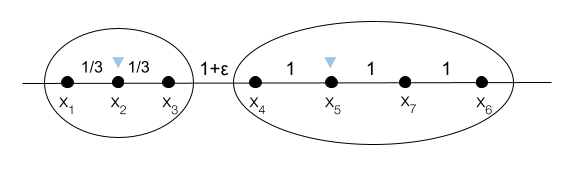
\includegraphics[width=\textwidth]{Images/nonStable2.png}
         \caption{Perturbed instance with the same clustering.}
         \label{fig:perOptCluster}
     \end{subfigure}
     \hfill
     \begin{subfigure}[b]{0.48\textwidth}
         \centering
         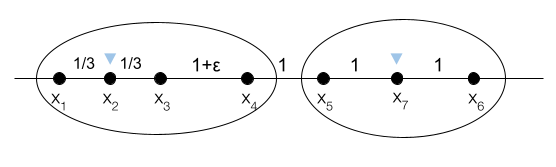
\includegraphics[width=\textwidth]{Images/nonStable3.png}
         \caption{Perturbed instance with an alternative clustering.}
         \label{fig:diffCluster}
     \end{subfigure}
      \caption{Example of non stable instance that satisfies all the properties.}
        \label{fig:NonStable}
\end{figure}



Never the less, the center-proximity is still a very important property. We can define the notion of $\g$-center stability. A instance is $\g$-center stable if in the optimal solution the center proximity holds for every point. This is a weak notion of stability since it allows more instances in the class. Figure \ref{fig:stability} illustrates all the different classes of stability.

\begin{definition}[$\g$-center stability]
A clustering instance $(X, d)$, with optimal solution $\CC= C_1, . . . , C_k$, is $\g$-center stable to a given objective function $\Phi$, if any $x_i\in C_i$ satisfies:
\[d(x_i,c_j) > \g d(x_i,c_i)\]
\end{definition}

\begin{figure}[ht]
    \centering
    
\includegraphics[width=11cm]{Images/stability.png}
    \caption{Classes of stable instances}
    \label{fig:stability}
\end{figure}




\section{Algorithms for Perturbation Stable Instances}

Τhe greater the factor of stability, the more structured the points are. For example, in every $2$-stable instance from weak center proximity, we get that every point is closer to its optimal center than any other point from  a different cluster. It is also very interesting that for a stability factor of $\g\ge2+\sqrt{3}\approx3.7$ we obtain from the separation property that all points are closer to all other points in their own cluster than to points in any other cluster. The next question is how we can use the properties derived from stability in order to achieve better results. The first idea is to see how existing algorithms perform on stable instances. \emph{Single-link} clustering is one of the most commonly used methods for clustering that uses the distances between the points. It starts with $n$ clusters of size $1$ (the data points), and at each step it merges the two clusters that have the minimum distance until there are $k$ clusters. One may think that if the instance is stable enough this algorithm could return the optimal solution, since at each step it connects the two ``closest" clusters. However, even in simple stable instances single linkage fails to find the optimal clustering. Consider an instance with 4 distinct locations $\x=(x_1,x_2,x_3,x_4)$. Our goal is to place $3$ facilities. There is one agent located at $x_1$ and $M>>1$ agents located at every other location. 

\begin{figure}[ht]
    \centering
    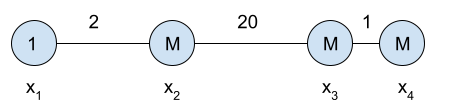
\includegraphics[width=13cm]{Images/SingleLinkageC.png}
    \caption{An example that single linkage fails to find the optimal solution}
    \label{fig:signleLinkage}
\end{figure}

The optimal solution is to place the centers at $x_2,x_3$ and $x_4$ and connect $x_1$ to the center at $x_2$. The total cost of the optimal solution is $2$. But the single-linkage clustering will merge the the clusters at $x_3$ and $x_4$ and places one center between them making total cost of the solution equal to $M$, which is arbitrarily larger than the optimal cost. Note that by construction the instance is $\g$-stable for arbitrarily large $\g$, for a properly selected value of $M$.  

But a variation of the previous algorithm can find the optimal solution for a sufficient $\g$ stability. It starts with $n$ clusters of size $1$. Instead of stopping at $k$ clusters it continues until one cluster remains. Then it finds the best $k$ clusters of the resulting tree $T$ using dynamic programming. 
%{?Write the dp?}

\begin{lemma}\label{sl}
Single linkage can find the optimal solution if and only if each cluster forms a subtree of the spanning tree. 
\end{lemma}

\begin{proof}
The single linkage algorithm outputs the best $k$-clustering among all the $\binom{n-1}{k-1}$ different choices. Every different clustering can be obtained by removing $k-1$ edges from the spanning tree. This way all the $k$ clusters are different connected components of  $T$, If some optimal cluster is not a connected subgraph of T the algorithm cannot find it.
\end{proof}
This can be illustrated with a simple example. 

\begin{figure}[ht]
    \centering
    
\includegraphics[width=9cm]{Images/MST.png}
    \caption{The optimal cluster $C_j$ do not form a subtree of $T$}
    \label{fig:my_label}
\end{figure}


The function used to determine the distance between two clusters, is known as the linkage function. For different functions we get different stability factors for which we can find the optimal solution. 

%--------------------------------------------------
% 3 & 2+sqrt(3)
The first linkage function was proposed by Awasthi \cite{Awasthi2012}. At each step it merges the two cluster $C,C'$ minimizing $d_{min}(C,C')$. The minimum distance between any two subsets $A,B \subset X$ is defined as:
\[ d_{min}(A,B) = min \{ d(a,b) | a\in A, b\in B\} \]

They prove that the single-linkage algorithm can return the optimal solution for a stability factor $3$ when centers must be data points and for stability factor $2+\sqrt{3}$ for general metrics. With tighter analysis Angelidakis showed \cite{Angelidakis2017} that the instance only needs to be $2$-metric stable, when the centers must be data points.

%From the Lemma \ref{sl}
\begin{lemma}
Single-linkage with $d_{min}$ as the linkage function finds the optimal solution in every $2$-metric stable instance. 
\end{lemma}

\begin{proof}
By Lemma \ref{sl} if every optimal cluster $C_i$ is a connected subgraph on the spanning tree $T$ then single-linkage returns the optimal solution. It is enough to show that the unique path that connects any point $a \in C_i$ to its optimal center $c_i$ on $T$ does not leave the cluster $C_i$. Suppose that $b$ is the next point on the path. Consider the step at which the single-linkage adds the edge $(a,b)$ to the spanning tree. At that step, $a$ and $c_i$ belonged in different clusters, otherwise the edge $(a,b)$ would form a cycle. We have that $d(a,b)<d(a,c_i)$ or else the edge $(a,c_i)$ would have been added instead of $(a,b)$. By Lemma \ref{WCprox} the previous inequality implies that $b$ belongs to $C_i$.  By induction all the points on the path between $a$ and $c_i$ belong to $C_i$.  
\end{proof}





%--------------------------------------------------
% 1+sqrt(2) center

The second linkage function was proposed by Balcan and Linang \cite{Balcan2011}. The single linkage algorithm merges the clusters with the minimum closure distance. The closure distance between two clusters $C,C'$ is the radius of the minimum ball that covers all the points in $C \cup C'$ and has some margin from points outside of the ball. A ball around $p$ with radius $r$ is set of all points that have distance from $p$ smaller than $r$: $\mathbb{B}(p,r) \coloneqq \{ q : d(p,q) <r \}$ 


\begin{definition}[Closure Distance]
The closure distance $d_S(C,C')$ between two disjoint nonempty subsets $C,C' \subset X$ is the minimum $d>0$ such that there is a point $c\in C\cup C'$ satisfying the following requirements:
\begin{enumerate}[(i)]
    \item Coverage: the ball $\mathbb{B}(c,d)$ covers $C$ and $C'$, that is, $C\cup C' \subseteq \mathbb{B}(c,d)$ 
    \item margin: points inside $\mathbb{B}(c,d)$ are closer to the center c than to points outside, that is, $\forall p \in \mathbb{B}(c,d), q\notin \mathbb{B}(c,d)$, we have $d(c,p)<d(c,q)$
\end{enumerate}

\end{definition}
\begin{lemma}
Single-linkage with $d_S$ as the linkage function finds the optimal solution in every $1+\sqrt{2}$-center stable instance. 
\end{lemma}

%\begin{proof}
%??????????
%\end{proof}

%This technique works because at each step every connected component is either a subset of a cluster in C, equal to C or a union of clusters in C. This is because the instance is stable and the algorithm always prefers to connect points that belong in the same cluster before connecting points from different clusters.




\section{Conclusion}

%Lower bounds
%approx stability 
%neg cant find how stable an instance is


Using the techniques from \emph{Beyond Worst Case Analysis} helps us avoid the hardness results in the general case. For clustering, we are able to design exact algorithms for a problem that is NP-hard to even approximate. However, the notion of perturbation stability does not completely solves our problem. There is an NP-hardness lower bound for the stability factor. For any $\epsilon>0$, finding the optimal $k$-center clustering for $(2-\epsilon)$-perturbation stable instances is $NP$-hard, unless $NP=PR$\cite{Balcan2015}. We also have that is $NP$-hard to find the optimal $k$-median clustering for $(2-\epsilon)$-center stable instances \cite{Ben-David2014}. Since the single-linkage algorithm only relies on the center proximity, which means the previous algorithm is tight. However, the class of $\g$-stable instances is a subclass of $\g$-center stable instances, which means that the lower bound does not transfer immediately. To show a lower bound for the class of $\g$-stable instances or to find a better algorithm, we need a different approach, specifically to include valid perturbations.

One downside of this approach is that there is no algorithm that can find or even estimate the  $\g$ for which an instance is $\g$-stable. However, the notion of $\g$-perturbation stability is still very important because it captures all the instances that have a ``clearly optimal" solution. That means we are clustering with the correct objective, which is not susceptible to minor perturbations.

%The class of $\g$-center stable instances includes all the instances for which in the optimal solution the $\g$-center proximity property holds. The class of $\g$-center stable instances includes the class of $\g$-perturbation stable instances since $\g$-center proximity is a necessary property for stability but not sufficient. ++++

%$(\g,\epsilon)$-perturbation stability, which states that at most a fraction $\epsilon$ of the total points can change cluster under any $\g$-perturbation.





\chapter{Facility Location on Perturbation Stable Instances}
%\section{Facility Location in Stable Instances}

In the previous section we saw that when we focus on the average instances of a problem, namely the "real-world" instances, we can avoid the hardness results and design better algorithms. Since clustering and facility location games are closely related problems, in this section we are going to see how perturbation stability in $k$-facility location games affects the design of mechanisms. Can we design strategyproof mechanisms with a bounded approximation ratio using the properties of stability? We have seen that in the simple setting where we want to locate $2$ facilities in the line any deterministic mechanism has $(n-1)$-approximation ratio because the agents have the power to change the clustering by misreporting their preferred location. So naturally it is very interesting to investigate the power any agent has in changing the structure of the clustering when the instance is stable and the clusters are well defined.


\section{Facility Location in Trees}


In this section, the agents are located in a Tree. With out loss of generality, we can view the tree with the location of agent $x_1$ as the root. We first need to adapt the definition of perturbation stability for the Facility Location games.

\begin{definition}[$\g$-Perturbation and $\g$-Stability]
Let $N$ be a set of $n$ agents located on a tree $(T,d)$, where $d$ is a metric distance function. Let $\x=(x_1,...,x_n)$ be a location profile. Let $\vec{z}= (z_1,...,z_m)$ denote the intersections on the tree, we will refer to them as phantom agents. A location profile $\xx=(x_1',...,x_n') \in (T,d')$ is a $\g$-perturbation of $\x$, for some $\g$, if for every pair of consecutive agents $x$ and $y$ (agents $x$ and $y$ can be any of $x_i-z_j$,$x_i-x_j$ or $z_i-z_j$ pairs) it holds:
\[ d'(x,y) \in  \bigg[\frac{1}{\g}d(x,y),d(x,y) \bigg]\]
 
A $k$-Facility Location instance $\x$, with optimal clustering $\CC=(c_1,...,c_k)$, is $\g$-(perturbation) stable, if for every $\g$-perturbation $\xx$ of $\x$ $\CC$ remains the unique optimal $k$-clustering.
\end{definition}


In order to properly define it we are going to assign phantom agents $\vec{z}=(z_1,...z_m)$ on every intersection of the tree. A $\g$-perturbation $\xx$ of an instance $\x$ can be obtained by scaling down any subset of pairs of consecutive agents, including the phantom agents, by a factor of at most $\g$. We can see that every valid metric-perturbation (Definition \ref{metricPer}) of the instance $\x$ (only agents' locations) can be performed by the process described above. Note that the distance between any pair of actual agents $x_i$ and $x_j$ is scaled down by a factor of at most $\g$ because the length of every pair of consecutive agents in the unique path that connects them is scaled down by a factor of at most $\g$. Moreover, the perturbed space is metric because the distance between $x_i$ and $x_j$ is the length of the unique shortest path between $x_i$ and $x_j$. Therefore, this class of $\g$-stable instances includes the class of $\g$-metric stable instances.  This notion of $\g$-perturbation captures all the perturbations that can be depicted on the same tree.

%We can perform every metric-perturbation but also perturbations that are not allowed by the definition for the clustering. For example we could scale down only the distance between an agent $x_i$ and a phantom agent $z_i$. 


\begin{figure}[ht]
    \centering
    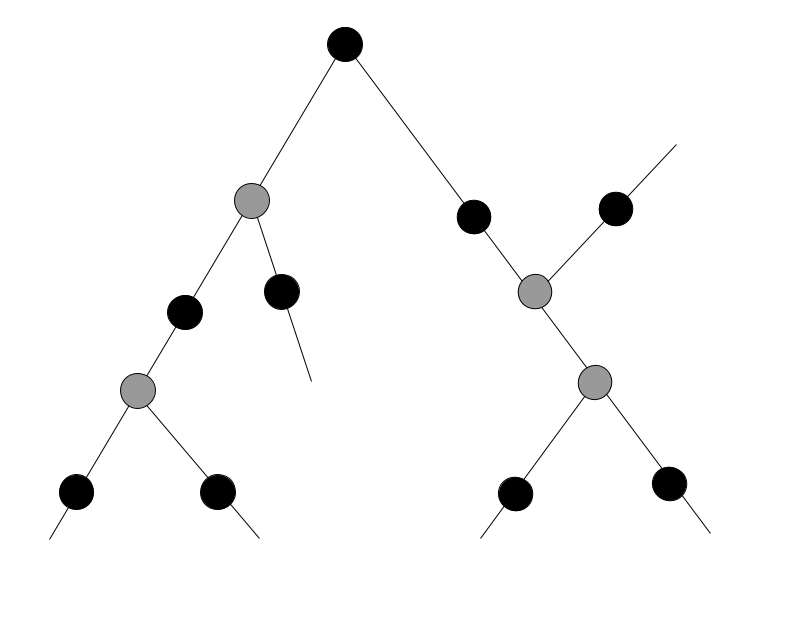
\includegraphics[width=8cm]{Images/Perturbation1.png}
    \caption{An example of a location profile $\x$ (black points) with phantom agents $\vec{z}$ on the intersections (gray points)}
    \label{fig:per}
\end{figure}



In the previous section, we showed that in general metric spaces in $\g$-stable instances, with $\g\ge2$, every cluster in the optimal solution forms a subtree in the minimum spanning tree. Similarly, we can show that this property holds when the underline metric space is a tree $T$. 
\begin{obs}\label{obs:subtrees}
Let $\x$ be a $\g$-stable, with $\g\ge2$, then in the optimal clustering $\CC$ every cluster $C_i$ forms a subtree.
\end{obs}

\begin{proof}
For contradiction suppose there exist a cluster $C_j$ that does not form a subtree, like in Figure \ref{fig:subtree}. Since the instance is stable we have that $d(x_{j_2},x_i)>(\g-1)d(x_{j_2},c_j)$. We also have that the distance between any two points is equal to the length of the unique path that connects those points, thus $d(x_{j_2},c_j) = d(x_{j2},x_i) + d(x_i,c_j)$. Using the previous inequality we get $d(x_{j_2},c_j)> (\g-1)d(x_{j2},c_j) + d(x_i,c_j) \implies d(x_i,c_j) < (2-\g) d(x_{j_2},c_j)$. When $\g\ge2$ the distance between $d(x_i,c_j)$ is negative but every distance function is non-negative.
\end{proof}

  
\begin{figure}[ht]
    \centering
    
\includegraphics[width=10cm]{Images/FCStableTree.png}
    \caption{Example of a cluster that does not form a subtree.}
    \label{fig:subtree}
\end{figure}



As we mentioned before, perturbation stability implies that there is a structure in the original location profile. In other words, the optimal solution is resilient to minor changes. In the facility location setting, the agents are strategic, which means they are motivated to misreport in order to reduce their connection cost. The idea is to see how much power a strategic agent has to change the outcome of a mechanism with a single deviation now that the instance has a well-defined optimal solution. Let us point out that an agent's deviation is entirely different from a perturbation of an instance. An agent can misreport at any location in the metric space, which may result in a non-stable instance. However, after a perturbation, the distance between any two agents is at most $\g$ times smaller than in the original instance. 

%\subsection{The Optimal solution is strategyproof for $(2+\sqrt{3})$-stable instances}
\subsection{The Optimal solution is strategyproof for \texorpdfstring{$(2+\sqrt{3})$}-stable instances}



\begin{algorithm}[ht]
\label{algorithm:optimal}
\DontPrintSemicolon
\SetAlgoLined
\LinesNumbered
\KwResult{An allocation of $k$-facilities}
\KwIn{A $k$-Facility Location instance $\x$.}
Compute the optimal clustering
 $(C_1, \ldots, C_k)$. Let $c_i$ be the median point of each cluster $C_i$.\;

 \uIf{\big($\exists i \in [k]$ with $|C_i|=1$\big) or \big($\exists \;x_i,x_i'\in Ci$ and  $x_j,x_j'\in C_j$ with $\max\{ d(x_i,x_i'), d(x_j,x_j')\} \geq d(x_i,x_j) $\big)}{
 \KwOut {``FACILITIES ARE NOT ALLOCATED''.}}\uElse{
 
\KwOut {The $k$-facility allocation $(c_1, \ldots, c_k)$ \;}}

\caption{\textsc{Optimal}}
\end{algorithm}

We next show that the the mechanism that returns the optimal solution is strategyproof for $(2+\sqrt{3})$-stable instances whose optimal clustering does not include singleton clusters. We need to exclude the stable instances with singleton clusters in their optimal solution from the mechanism because there is always an agent that can benefit by becoming a singleton cluster. Consider a $\g$-stable instance $\x$. Suppose an agent $x_i \in C_i$ reports a location $x'$ far away from any location in $\x$ creating a different instance $\x\,'$. Since the mechanism allocates the facilities optimally $x'$ becomes a singleton cluster. Now the mechanism has to allocate $k-1$ facilities to the remaining agents, which means two clusters from the original optimal solution merge. We can always create an instance in which cluster $C_i$ merges with its neighbor cluster $C_j$ which makes the new median closer to $x_i$. The main problem is that the new instance $\x\,'$ is also $\g$-stable as the original and there is no way to determine whether or not there is a deviation. 


\begin{figure}[ht]
    \centering
    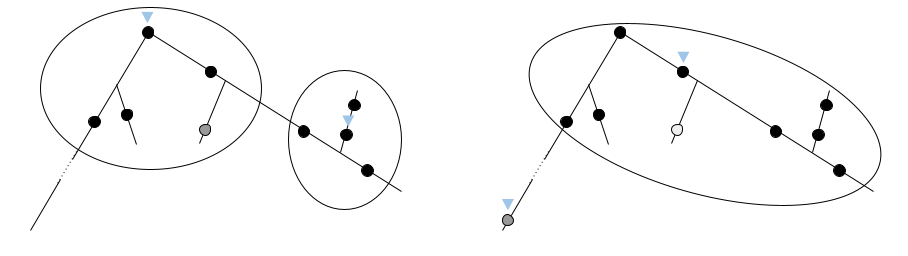
\includegraphics[width=\textwidth]{Images/singleton.png}
    \caption{Singleton Deviation}
    \label{fig:singleton}
\end{figure}

It is also important to remember that we cannot efficiently estimate the stability factor of a given instance. This is why we rely on the properties that derive from stability, since the properties are necessary but not sufficient for stability. That also means that the mechanism serves instances that are non-stable but satisfy the cluster separation property. We can efficiently check if the cluster separation property is violated between any to clusters. Since every cluster in the optimal solution forms a subtree, we only have to check if any of the $k-1$ edges between 2 different clusters violates the cluster separation property.


\begin{theorem}
The \textsc{Optimal} Mechanism applied to $(2+\sqrt{3})$-stable instances of $k$-Facility Location without singleton cluster in their optimal clustering is strategyproof and minimizes the social cost. 
\end{theorem}


%proof optimal
\begin{proof}
The mechanism returns the optimal solution, so we only need to prove that it is strategyproof. Let any $(2+\sqrt{3})$-stable instance with optimal clustering $\CC = (C_1,..., C_k)$. Suppose agent $x_i \in C_i$ reports a location $y$ in order to decrease her cost. Let $\y = (\x_{-i},y)$ be the instance after the deviation, and $\Y$ be its optimal clustering.There are three possible deviations:
\begin{enumerate}[1.]
    \item If $y$ is in the area of $C_i$, then the clustering structure would not change. But the median location for one facility on trees is strategyproof and thus she cannot benefit from such deviation.
    \item If $y$ is a singleton cluster in $\Y$, then the mechanism would not allocate any facilities, making her cost infinite times larger.
    \item If $y$ is cluster together with agents from different clusters in $\CC$. 
\end{enumerate}

We will only focus on the third case since this is the only way she could benefit. In order for the mechanism to be strategyproof, we need to show that either the deviation is not profitable ($d(x_i,\CC) < d(x_i,\Y)$) or that the cluster separation property is violated and no facilities are allocated. 

We have that $y$ is clustered together with agents belonging in one or two clusters of $\CC$, let that clusters be $C_j$ and $C_l$. In $\Y$ the number of facilities serving agents from $C_j\cup C_l \cup \{y \}$ are at least the number of facilities serving agents from $C_j\cup C_l$ in $\CC$, because both $\CC$ and $\Y$ are optimal clusterings. Suppose one facility is placed to an agent in $C_j$. The original instance is $2+\sqrt{3}$-stable, so by the separation property we have that every agent is closer to every agent from her own cluster that to any other agent from a different cluster. This implies that no agent in $C_j$ is served by a facility in $\x\setminus C_j$. 
 
\begin{description}
\item[Case 1:] \textit{ $y$ is not allocated a facility in $\Y$}: This can happen in one of two ways:
    \begin{description}
        \item[Case 1a:] $y$ is clustered together with some agents from cluster $C_j$ and no facility placed in $C_j$ serves agents in $\x\setminus C_j$ in $\Y$. 
        
        \item[Case 1b:] $y$ is clustered together with some agents from a cluster $C_j$ and at least one of the facilities placed in $C_j$ serve agents in $\x\setminus C_j$ in $\Y$.
\end{description}
        
\item[Case 2:] \textit{$y$ is allocated a facility in $\Y$}. This can happen in one of two ways:

 \begin{description}
        \item[Case 2a:] $y$ only serves agents that belong in $C_j$ (by optimality, $y$ must be the median location of the new cluster, which implies that either $y$ is not in the area of $C_j$ and only serves one agent from $C_l$ or $y$ is in the area of $C_j$ and serves multiple agents).
        \item[Case 2b:] In $\Y$, $y$ serves agents that belong in both $C_{j-1}$ and $C_j$.
\end{description}
\end{description}

We first consider the cases 1a and 2a, namely the cases where in $\Y$ there is a facility in $C_j$ that only serves agents in $C_j$. If there is only one facility allocated in $C_j\cup\{y\}$ then both clusterings $\CC$ and $\Y$ have the same structure, making $x_i$'s deviation not profitable. So, in $\Y$ there must be two facilities in $C_j\cup\{y\}$. Suppose there is a location $y$ such that the deviation is profitable, $d(x_i,\CC) > d(x_i,\Y)$. Since $\Y$ is the optimal clustering for $\y$ we have that:
\begin{align*}
    cost(\y,\CC) &> cost(\y,\Y) \iff \\
    cost(\x,\CC) + d(y,\CC) - d(x_i,\CC) &> cost(\x,\Y) + d(y,\Y) - d(x_i,\Y) \iff \\
    d(y,\CC) - d(y,\Y) &> cost(\x,\Y) - cost(\x,\CC)  + d(x_i,\CC) - d(x_i,\Y)
\end{align*}

Since $i$'s deviation to $y$ is profitable ($d(x_i,\CC) - d(x_i,\Y)>0$) we get:

\begin{align}
\begin{split}
d(y,\CC) - d(y,\Y) &> cost(\x,\Y) - cost(\x,\CC)\label{eq:gainy} \\
&= cost(C_j,\Y)-cost(C_j,\CC)-cost(\x\setminus C_j,\Y)-cost(\x\setminus C_j,\CC)
\end{split}
\end{align}


    
%{???}

We now consider a valid $\gamma$-perturbation $\xx$ of the original instance $\x$: We first remove from the instance all the agents from $C_j$ and all the edges connected to them. This may break the instance in more than one connected components. By observation \ref{obs:subtrees}, we have that there is no cluster whose agents belong in more than one connected components. Then, we scale down by $\g$ all the distances between consecutive agents that are in the same connected component. By stability, the clustering $\CC$ remains the unique optimal clustering for $\xx$ therefore $cost(\xx,\CC) < cost(\xx,\Y)$. Since, in cases 1a and 2a, the facility allocated to an agent of $C_j\cup \{y\}$ does not serve agents in $\x \setminus C_j$ in $\CC$ and $\Y$ we have:
\begin{align*}
 cost(\xx, \CC) = cost(C_j,\CC)+\frac{1}{\gamma}cost(\x\setminus C_j,\CC)\\
 cost(\xx, \Y) = cost(C_j,\Y)+\frac{1}{\gamma} cost(\x\setminus C_j,\Y)
\end{align*}
Using that $cost(\xx,\CC) < cost(\xx,\Y)$ and  that for any $\gamma\ge2$ it holds $\frac{1}{\gamma} \le 1-\frac{1}{\gamma} $ we get:
\begin{align}
   cost(C_j,\CC) - cost(C_j,\Y) &< \frac{1}{\gamma} \left( cost(\x\setminus C_j,\Y) - cost(\x\setminus C_j,\CC) \right)\label{eq:costIneq1} \\
    &\le (1 -\frac{1}{\gamma}) \left( cost(\x\setminus C_j,\Y) - cost(\x\setminus C_j,\CC) \right) \label{eq:costIneq}
\end{align}

Rearranging (\ref{eq:costIneq}) we get:
\begin{equation}
    cost(\x,\Y) - cost(\x,\CC) > \frac{1}{\gamma}\left( cost(\x\setminus C_j,\Y) - cost(\x\setminus C_j,\CC) \right)\label{eq:lowerBcostY}
\end{equation}

%{?????????????}
 
%To prove the previous inequality it suffice to show that the decrease in the cost of $y$ due to the additional facility in $\Y$ is at most the decrease in the cost of an agent from $C_j$ in $\Y$.
We know that there are at least two facilities serving $C_j\cup\{y\}$. Let $Y_{j_1}$ be the cluster that contains $y$ and some agents of $C_j$. In case 1a, let $x_j \in Y_{j_1}$ be the agent that has the facility. Then the decrease in the cost of $y$ due to the additional facility in $\Y$ is at most the decrease in the cost of an agent from $C_j$ in $\Y$. In case 2a, where agent $y$ has a facility, by optimally of $\Y$, we have that $y$ is the median of the new cluster. If we view $c_j$ as the root of the tree then $y$ has at least one agent from $C_j$ as a child; otherwise it would not be the median location. Therefore, the decrease in the cost of $y$ is at most the decrease in the cost of an agent from $C_j$ in $\Y$. (The case where $y$ is not in the area of $C_j$ and only serves one agent is equivalent to placing the facility on the other agent and serving $y$ from there). In both cases, we can bound from below the total decrease in the cost of $C_j$ due to the additional facility.

\begin{align*}
   d(y,\CC)-d(y,\Y)  &\le cost(C_j,\CC)-cost(C_j,\Y) \xRightarrow{(\ref{eq:costIneq1})}\\
   &\le \frac{1}{\gamma} \left( cost(\x\setminus C_j,\Y) - cost(\x\setminus C_j,\CC) \right) \xRightarrow{(\ref{eq:lowerBcostY})}\\
   &< cost(\x,\Y) - cost(\x,\CC)
\end{align*}

Which contradicts equation (\ref{eq:gainy}).


%---------------------------------------------------------------------------------------------

\bigskip

Now we consider cases 1b and 2b, namely the cases where some agents of $C_j$ are clustered with agents of $C_l$. Let $Y_{j_1}$ and $Y_{j_2}$ denote the clusters of $\Y$ that include all the agents of $C_j$. Let $Y_{j_1}$ be the cluster that has agents from $C_j$ and $C_l$. Consider $x_1 \in Y_{j_1} \cap C_j$, $z\in Y_{j_1} \cap C_l$ and $x_2 \in Y_{j_2}\cap C_j$. By the cluster separation property $d(x_1,z) \ge D_{x_1}$, where $D_{x_1}$ is the largest intra-cluster distance from $x_1$. Since $x_1$ and $x_2$ belong in the same cluster in $\CC$ we have that $d(x_1,x_2)<D_{x_1}$. Therefore, $d(x_1,z)>d(x_1,x_2)$ which violates the cluster separation property, since an intra-cluster distance is greater than an inter-cluster distance. In this case, the mechanism will not allocate any facilities. 
\end{proof}


\iffalse
\section{Lower bound on stability }




\begin{theorem}
For every $k\ge3$ and $\delta>0$, any deterministic anonymous strategy proof mechanism for $(\sqrt{2}-\delta)$-stable instances of $k$-facility location on the line with $n\ge k+1$ agents has an unbounded approximation ratio.
\end{theorem}
\fi
%----------------------------------------------------------------------------------------------

%\section{General metrics}
%\subsection{The \textsc{Random} mechanism is strategyproof for 5-Stable instances}

%\begin{theorem}

\end{theorem}

\begin{proof}
Let $\vec{x}$ be any $5-$stable instance with optimal clustering $\vec{C} = (C_1,...,C_k)$. Let $\vec{x}' = (\vec{x}_{-i},x')$ be the resulting instance after agent $i$ deviates from location $x_i$ to $x'$, with optimal clustering $\vec{C'}$. In the original clustering $x_i\in C_i$. Since the mechanism places a facility at a location of an agent selected uniformly at random from each optimal cluster, no agent can gain by deviating within the range of her optimal cluster. Therefore we need to cover all $i$'s possible deviations that result in a different clustering than the original. This can happen in three ways:

\begin{itemize}
\setlength\itemsep{0.1em}
  \item[]\textbf{Case 1:} Becoming a member of another cluster
  \item[]\textbf{Case 2:} Becoming a self serving cluster
  \item[]\textbf{Case 3:} Merging or splitting $C_i$
\end{itemize}


In case 1, agent $i$ is clustered together with members from a different cluster in $\vec{C}$ without splitting or merging $C_i$. The deviation from $x_i$ to $x'$ results in either an increase in her expected cost or a violation of the cluster separation property in $\vec{C}'$.


First, we need to compute the expected $i$'s cost if she reports her true location. We can define as $X_i$ the discrete random variable that takes values from the sample space $\{ d(x,x_i): x\in C_i\}$ uniformly at random. Let $|C_i|=n$. Then, her expected cost is:

\[ E[X_i] = \frac{\sum_{x\in C_i} d(x,x_i)}{n} \]

Note that $i$'s cost is at most $D(C_i)$ since the center is selected uniformly at random among the agents in $C_i$.



In this case, agents in $C_i$ are not merged or splitted in $\vec{C}'$. So, all the agents that were originally cluster together with $x_i$ in $\vec{C}$ are cluster together in $\vec{C}'$. Let that be $C_i'$. %($x\in C_i\setminus x_i$) 
%needs haaalp!!
Let $C_j'$ be the cluster that $x_i$ belongs in $\vec{C}'$. Since she is trying to make the deviation profitable $C_j'$ need to be the closest cluster, different from $C_i'$, to her original location.


After this change in the clustering we need to compute $i$
's expected cost. Same as before, we can define as $X_i'$ the discrete random variable that takes values from the sample space $\{ d(x,x_i): x\in C_i' \}  \equiv \{ d(x,x_i): x\in C_i, x\neq x_i \}$ and $X_j'$ the discrete random variable that takes values from the sample space $\{d(x',x_i)\} \	\cup \{ d(x,x_i): x\in C_j'\}$ uniformly at random. $X_i'$ represents $i$'s cost if she is served by the facility placed in $C_i'$ and $X_j'$ her cost if she is served by the facility in $C_j'$. Her expected cost becomes $\mathbb{E} [min\{ X_i', X_j' \}]$, since she can choose the facility closest to $x_i$. 
By the cluster separation property for any agent $x_j \notin C_i$ it holds that $d(x_i,x_j)>D(C_i)$.  We know that: 
\[\mathbb{E}[X_j'] =  \frac{\sum_{x \in C_j'} d(x,x_i) + d(x',x_i)}{|C_j'|+1}\]

If $d(x_i,x') > D(C_i)$ then all the values from $X_j'$'s sample space are larger than  $X_i$'s. Thus, agent i will always has small expected cost if she chooses the facility placed in $C_i'$. 
\[\mathbb{E}[min\{X_i',X_j'\}] = \mathbb{E}[X_i'] = \frac{\sum_{x \in C_i'} d(x,x_i)}{n-1} = \frac{\sum_{x \neq x_i\in C_i} d(x,x_i)}{n-1} > \mathbb{E}[X_i]\]

Since she is not a member of $C_i'$ she cannot affect the facility's location, making her expected cost higher than her original expected cost.
\bigskip

The only way she can gain by the deviation is if $x'$ belongs in $C_j$ and $d(x',x_i)<D(C_i)$. This way, she is close enough to her original location to make the deviation profitable but far enough to change the original clustering. Consider the case where $c_i$, $x_i$ and $x_j$ are collinear, $x_j$ being the agent from $C_j$ closest to $x_i$. In any other case, the distance $d(x',C_i')$ will be smaller, making the deviation easier to detect. 

By the cluster separation property for the stability factor of $5$, we have that  $d(x_i,x_j) = d(C_i,C_j) \ge 1.6\cdot D(C_i)$. In order for this distance to be tight all it must be $d(x_i,c_i) = 0.4D(C_i)$. We also have that $d(x_j,c_j) < 0.4D(C_i)$, since by stability it holds $d(x_i,x_j) > (\gamma-1)d(x_j,c_j)$. Combining the above inequalities and that $d(x',x_i)<D(C_i)$ we get:
\begin{align}
d(x',c_i) \le d(x',x_i) + d(x_i,c_i) \le 1.4D(C_i) \\
d(x',x_j)>d(x_i,x_j) - d(x_i,x') > 0.6D(C_i)
\end{align}


Finally we need to distinguish two cases regarding the cluster $C_j'$: 
\begin{enumerate}
    \item $c_j \in C_j'$:  We have that $D(C_j') \ge d(c_j,x')$ and that $d(C_i',C_j') \le d(c_i,x') \le 1.4 D(C_i)$. By stability it hold $d(x_i,c_j) > \gamma d(x_i,c_i) = 2D(C_i)$. From triangle inequality it holds $d(c_j,x') \ge  d(c_j,x_i)-d(x_i,x') > D(C_i)$. Therefore, we get that $d(C_i',C_j') \le 1.4 D(C_i) < 1.4 D(C_i')$ 
    
    \item $c_j \notin C_j'$: In this case the agents from $C_j$ are splitted in (at least) two clusters in $\vec{C}'$. Let $C_l'$ be the cluster than $c_j$ belongs to. Since $x_j\in C_j'$ and $c_j \in C_l'$ we have that $d(C_j',C_l') \le d(c_j,x_j) < 0.4D(C_i)$. But $D(C_j') \ge d(x_j,x')>0.6D(C_i)$. Combining this inequalities we get $D(C_j',C_l') \le 0.67 D(C_j')$ which violates the minimum distance between  $C_j'$ \& $C_l'$.
\end{enumerate}

\end{proof}




\section{Conclusion and Future Work}
Remember that without making any assumptions about the instance, we cannot design strategyproof mechanisms with a bounded approximation because we cannot identify the optimal clusters in a strategyproof way. However, if we focus on perturbation stable instances, the structure helps us avoid that problem. Now we can efficiently find the optimal solution and place the facilities within each optimal cluster. We also showed that the strategic agents do not have the power to change the structure of the instance for a stability factor $\g\ge2+\sqrt{3}$ because all the inter-cluster distances are greater than the intra-cluster distances. This allows us to reduce the multi-facility location games on stable instances to a one-facility location game and use all the known results.

In the \textsc{Optimal} mechanism, we saw that we have to exclude the instances that contain singleton clusters because an agent can deviate to a location far away and bring a facility closer to her true location (singleton deviation). One way to overcome this problem is to limit the range of possible locations each player can declare based on their actual locations. In this case, we must also see how stable the instance must be in order for the optimal solution to be strategyproof.

Another direction is to assume a ``weaker" notion of stability in the instances. In the literature, $(\g,\epsilon)$-perturbation stability was also proposed, which states that at most $\epsilon n$ total points can swap into or out of each cluster under any $\g$ perturbation. These instances are more likely to describe ``real world"  instances. However, the non-stable points may be harder to handle.








%\chapter{Future Work}
%%In the optimal mechanism we need excluded all the instances in which the optimal clustering includes singleton clusters because there is now way to distinguish 


\bibliographystyle{./Bibliography/IEEEtranS}
\bibliography{./Bibliography/myBib}

\end{english}


\end{document}
